\chapter{$\Dsplus$ production in pp collisions at $\s$ = 7 TeV}

The 7 TeV sample is the one providing up to now the most precise pp reference of
the nuclear modification factors $\RAA$ and $\RpPb$. 
Furthermore, it constitutes a benchmark for pQCD predictions
at this energy.
In comparison to previous ALICE publications based on the same data 
sample~\cite{ALICE:2011aa,Abelev:2012tca,Adam:2016ich}, the present 
results have total uncertainties reduced by a factor of about two. This improvement 
has several sources: 
\begin{itemize}
\item changes in the detector calibration, alignment and track reconstruction 
algorithm, which resulted in better $\pt$ resolution, thus higher signal-to-background ratio; 
\item optimization of the D-meson selection procedure; 
\item refinements in the estimation of the systematic uncertainties, which is now more data-driven;
\item a data sample with 20\% larger integrated luminosity.
\end{itemize} 
Events are selected requiring a primary vertex reconstructed from ITS+TPC tracks with 
$z$-vertex coordinate $|z_{\rm RecoVert}|<~10$~cm, 
and pile-up events are rejected.  
The number of analysed events is 370M, while it was 300M for the previous reconstruction.

\section{$\Dsplus$ reconstruction and strategy}
The transverse momentum spectra of prompt charm-strange meson 
$\Dsplus$ was measured in the rapidity range $|y| < $0.5 in pp collisions at 
$\sqrt{s}$ = 7 TeV with the ALICE detector.\\
The $\Dsplus$ mesons can not be directly detected because of 
their mean proper decay length $c\tau = 150\pm 2$ $ \mu$m~\cite{Olive:2016xmw} 
that prevent them from reaching the detectors. Hence, the analysis is 
based on the reconstruction of the full decay chain.
$\Dsplus$ mesons and their antiparticles were 
 reconstructed in the decay channel $\Dstophipi$ 
 (and its charge conjugate) followed by $\PhitoKK$ 
 (Fig.~\ref{fig:DsDecayTopology}). The branching ratio (BR) of this decay channel 
 is 2.27 $\pm$ 0.08 \%~\cite{Olive:2016xmw}.
Other $\Dsplus$ decay channels can give rise to the same final products
 $\KKpi$, such as $\Dsplus\rightarrow {\rm  K^{*0} K^+}$ and 
 $\Dsplus\rightarrow f_o(980) \pi^+$ with BR  2.63 $\pm$ 0.13 \% and 
 1.16 $\pm$ 0.32 \%, respectively. It was verified that the selection efficiency for 
 these decay modes is strongly suppressed by the cuts applied 
 to select the signal candidates of $\DstophipitoKKpi$, that include 
 a selection exploiting the mass of the intermediate resonant state. 
 Since the width of the $\phi$ peak is narrower than those of the 
 K$^{*0}$ and the $f_o(980)$, the decay channel through the 
 $\phi$ resonance, being the one that provides the best discrimination 
 between signal and background, was used in this analysis. 
 The $\Dsplus$ signal is extracted from 
 the invariant-mass\footnote{The invariant mass equation is \\ 
 \begin{align*} m^2 =& E^2 -\vec{p}^{\, 2} = (E_1 + E_2)^2 -(\vec{p_1} + \vec{p_2})^2 \\ m^2 =& m_1^2 +m_2^2 + 2(E_1E_2 -p_1p_2cos\theta) \end{align*}} 
 distribution of the candidates, which are obtained by 
 combinatorial association of three reconstructed tracks with the correct 
 charge-sign combination. Hence, 
 the invariant-mass distribution will have a contribute from real 
 $\Dsplus$ decays ($\DstoKKpi$) and an other 
 from combinatorial background of uncorrelated tracks. In order to have a reduction of the
  background, specific cuts were applied on the decay topology, on
   the invariant mass of $\KK$ pair and on the particle identification, 
   as explained in the following sections. 
$\Dsplus$ meson mean proper decay length of $\sim 150\, \mu$m  
makes it possible to separate their decay vertex from the primary vertex
of the pp interaction. 
This gives a fundamental contribution in rejecting tracks which do not come from a displaced vertex.
\begin{figure}[!t]
\centering
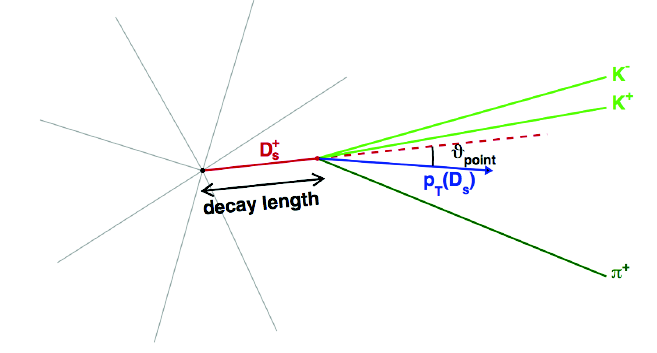
\includegraphics[width=12cm]{FigCap4/Ds.png}
\caption{Schematic view of the $\Dsplus\rightarrow \phi \pi^+ \rightarrow K^+K^-\pi^+$ decay.}
\label{fig:DsDecayTopology}
\end{figure}
Before the candidates go through specific selections of the decay
topology and particle identification, they have to pass single-track 
quality cuts. In the following, details of each selection step will
be illustrated. 



\section{Single-track selections}
Reconstructed tracks were selected by requiring:
\begin{itemize}
\item pseudo-rapidity $|\eta| < 0.8$
\item minimum $\pt > 0.3~\GeV/c$
\item at least 70 (out of a maximum of 159, i.e. number of TPC pad rows) 
associated space points in the TPC
\item $\chi^2/\mathrm{ndf} < 2$ in the TPC (where ndf is the number of degrees of 
freedom involved in the tracking procedure)
\item at least two (out of six) hits in the ITS, out of which at least one 
in either of the two SPD layers
\item ratio of crossed rows (total number of hit pad rows, corrected 
for pad rows with missing signal) over findable clusters (pad rows which, 
based on the geometry of the track, are possible clusters) in the TPC larger than 0.8
\end{itemize}
For tracks that satisfy the above selection criteria, the transverse momentum 
resolution is better than 1$\%$ at $\pt = 1\, \Gevc$ and about 2\% at $\pt = 10 \, \Gevc$. 
The resolution on the track impact parameter, which is the distance of closest 
approach of the track to the primary vertex, is better than 75 $\mu$m for 
$\pt >$ 1 $\Gevc$ for the projection on the bending plane ($r\phi$, normal to 
the beam direction) in pp collisions.
In order to have unbiased determination of the primary vertex, for each 
$\Dsplus$ candidate the interaction point was recalculated from the reconstructed 
tracks after excluding the candidate decay tracks.
\begin{figure}[!htbp]
\begin{center}
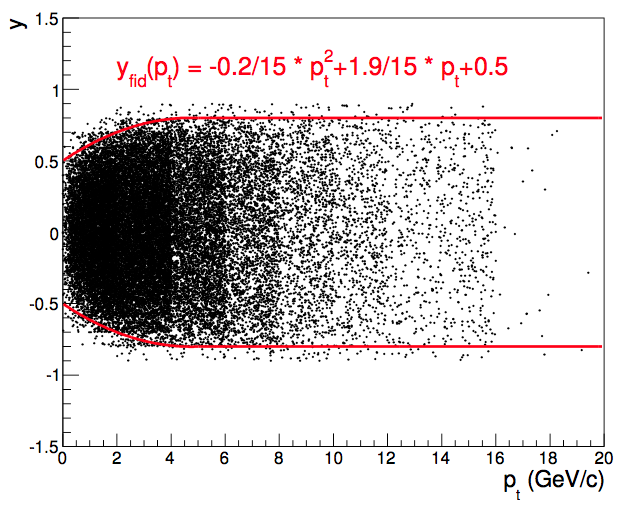
\includegraphics[width=.5\textwidth]{FigCap4/YvsPt.png}
\label{fig:singtrafter}
\caption{Rapidity versus $\pt$ distribution of the reconstructed $\Dsplus$ mesons. The fiducial acceptance region is defined by $|y| < y_{fid}(\pt)$.}
\end{center}
\end{figure}

The single-track selection criteria reduce the $\Dsplus$-meson acceptance, which drops 
steeply to zero for $|y| > 0.5$ at low $\pt$ and for $|y| > 0.8$ 
at $\pt > 5~\Gevc$. A $\pt$-dependent fiducial acceptance region was therefore defined as 
$|y| < y_{\mathrm{fid}}(\pt)$, with $y_{\mathrm{fid}}(\pt)$ increasing 
from 0.5 to 0.8 in the transverse momentum range $0 < \pt < 5~\Gevc$ 
according to a second-order polynomial function, and $y_{\mathrm{fid}}=0.8$ 
for $\pt > 5~\Gevc$.

\section{Decay-chain and topology selection}

The single-track selection provided a certain number of candidate
 decay tracks. Then, $D^{\pm}_s$ candidates were build from combinatorial 
 association of three candidate tracks, with the correct combination of charge 
 sign. In this way, a huge number of candidates was created, most of them 
 being combinatorial background. The goal is to separate background from
  $D^{\pm}_s$ signals (i.e. corresponding to real  $D^{\pm}_s$ decays). Candidates 
  are thus selected by applying topological cuts, specific to the meson and its 
  decay channel and varying as a function of the D meson $\pt$.
The main feature of the $\Dsplus$-decay topology is the presence of three tracks displaced from 
the primary vertex and compatible with the hypothesis of being originated from 
a common point. 
The variable that allows one to evaluate the displacement of a track is the 
impact parameter. The two most important detectors for the measurement
 of the impact parameter are the two SPD inner layers of the Inner Tracking System. \\
Below, the topological cuts used for $D^{\pm}_s$ signal selection
 are explained in detail. Fig.~\ref{fig:var1},~\ref{fig:var2},~\ref{fig:var3} complement
 the description, showing distributions of some of the below listed variables
 for signal and background candidates, in the interval $2 < \pt < 16 \, \Gevc$, 
 extracted from Monte Carlo production (PYTHIA~\cite{Sjostrand:2006za}) and data, respectively.
  New topological variables were introduced with respect to the 
  previous analysis of the same sample. They are the projections of the cosine of 
the Pointing angle and of the (normalised) decay length in the $xy$ plane 
 and the single-track normalised impact parameter residual.
\begin{itemize}
\item \textbf{Decay length $D_{len}$}, defined as the distance between
 primary and secondary vertex. $\Dspm$ decay vertexes are displaced by
  a few hundred $\mu$m from the interaction vertex. Since real $\Dspm$ 
  decay vertices have, on average, larger values of decay length than the
   background, this allows one to discriminate signal from background. 
   Likely cut values are $D_{len} > 300-400\, \mu $m. Fig.~\ref{fig:var1} (left) 
   shows distribution of $D_{len}$ for background and signal candidates.
   To be noted that candidates coming from weak decays of beauty hadrons have larger $D_{len}$
   with respect to prompt $\Ds$ from charm decay, due to more displaced decay vertices.
\item \textbf{Normalized decay length $L$}, defined as the decay length 
divided by its uncertainty (Fig.~\ref{fig:var1} right).
\item \textbf{Cos$\theta_{point}$}, where $\theta_{point}$ is the angle
 between the momentum of the reconstructed $\Dspm$ meson and the 
 $\Dspm$ flight line (line connecting primary and secondary vertex, see
  left panel in Fig.~\ref{fig:var2}). The pointing angle is expected to be small for signal 
  candidates, resulting in a distribution of cos$\theta_{point}$ peaking at 1 for 
  signal and being broader for background candidates. Hence, cuts like 
  cos$\theta_{point} >$ 0.93 or tighter were usually applied to reject background.
\begin{figure}[!t]
\centering
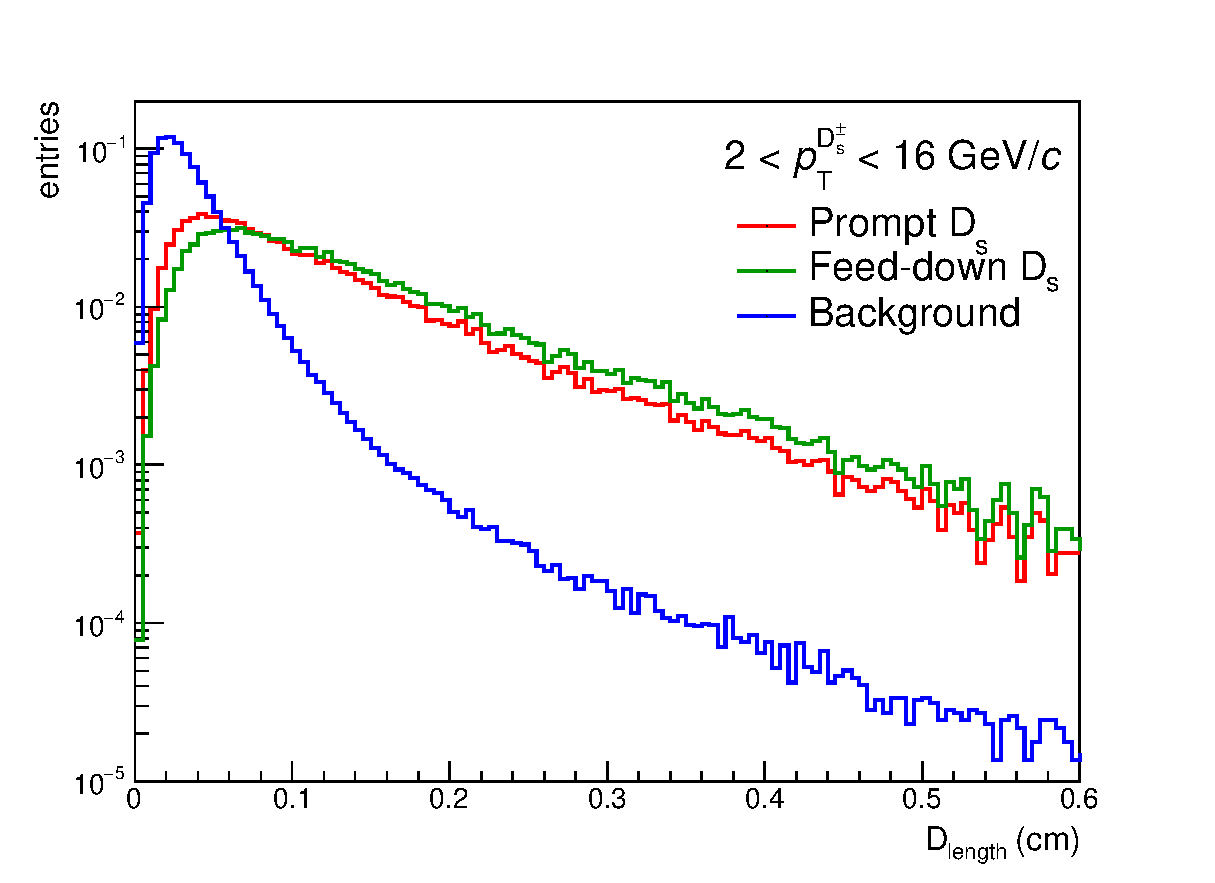
\includegraphics[width=6.5cm]{FigCap4/DL.eps}
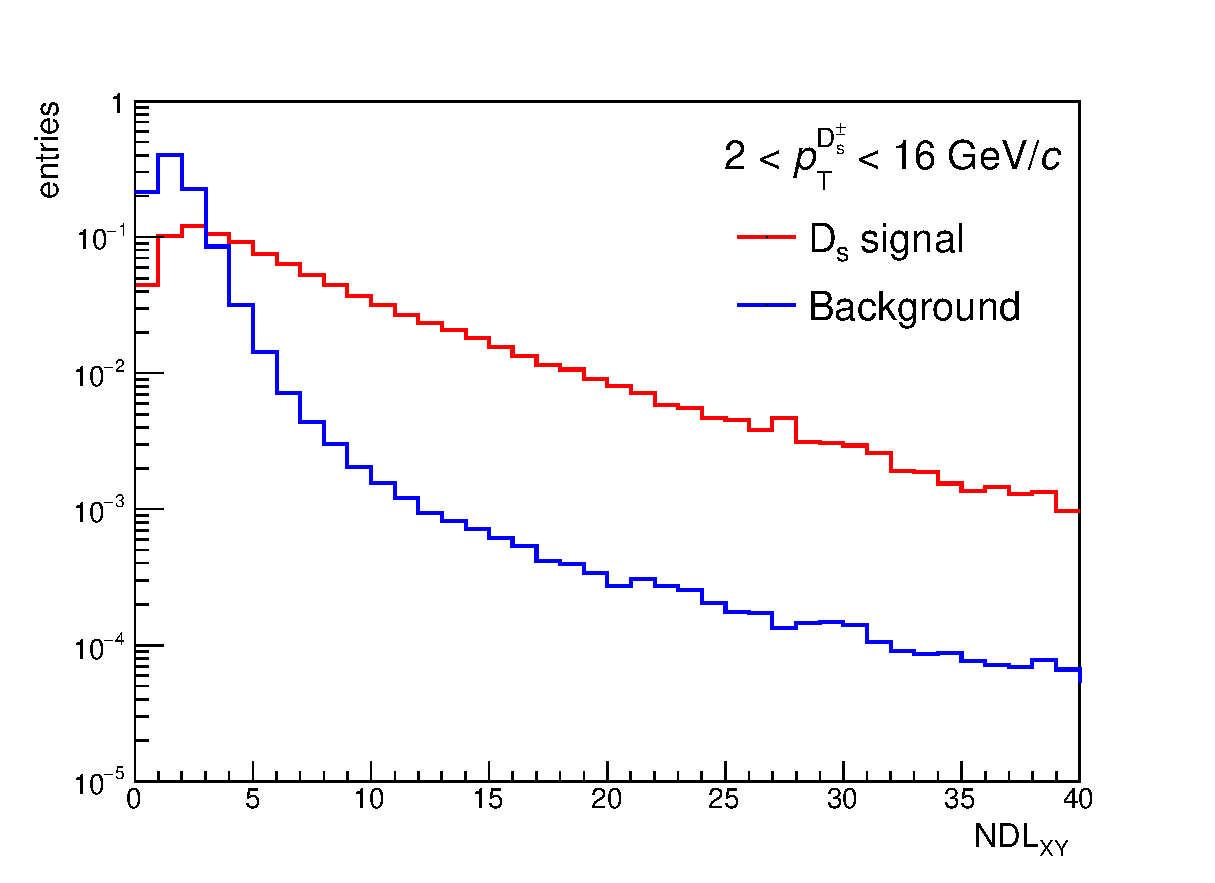
\includegraphics[width=6.5cm]{FigCap4/NDLxy.eps}
\caption{Left: distributions of decay length for prompt (red), feed-down (green) signal and background (blue) $\Ds$ candidates. Right: distributions of normalised decay length in the transverse plane signal (red) and background (blue) $\Ds$ candidates.}
\label{fig:var1}
\end{figure}
\begin{figure}[!h]
\centering
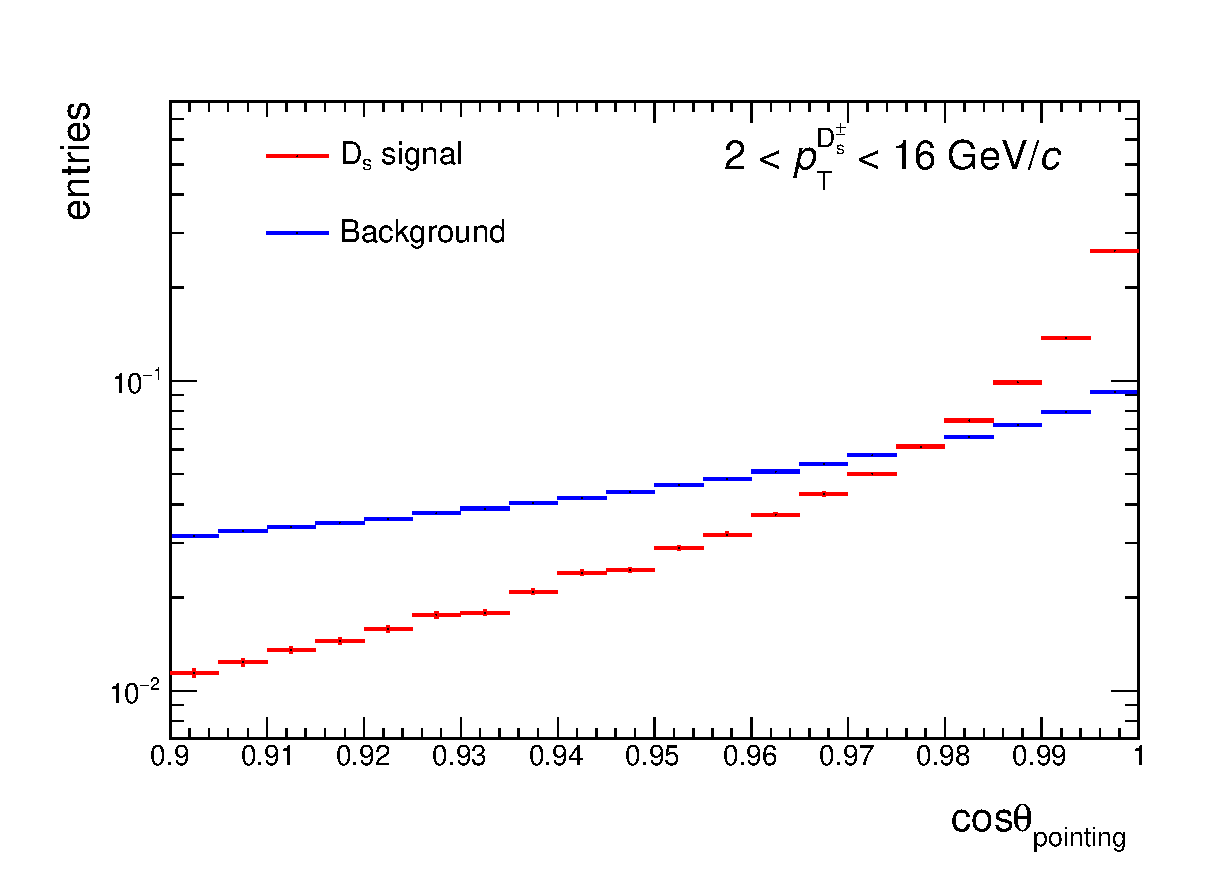
\includegraphics[width=6.5cm]{FigCap4/cosP.eps}
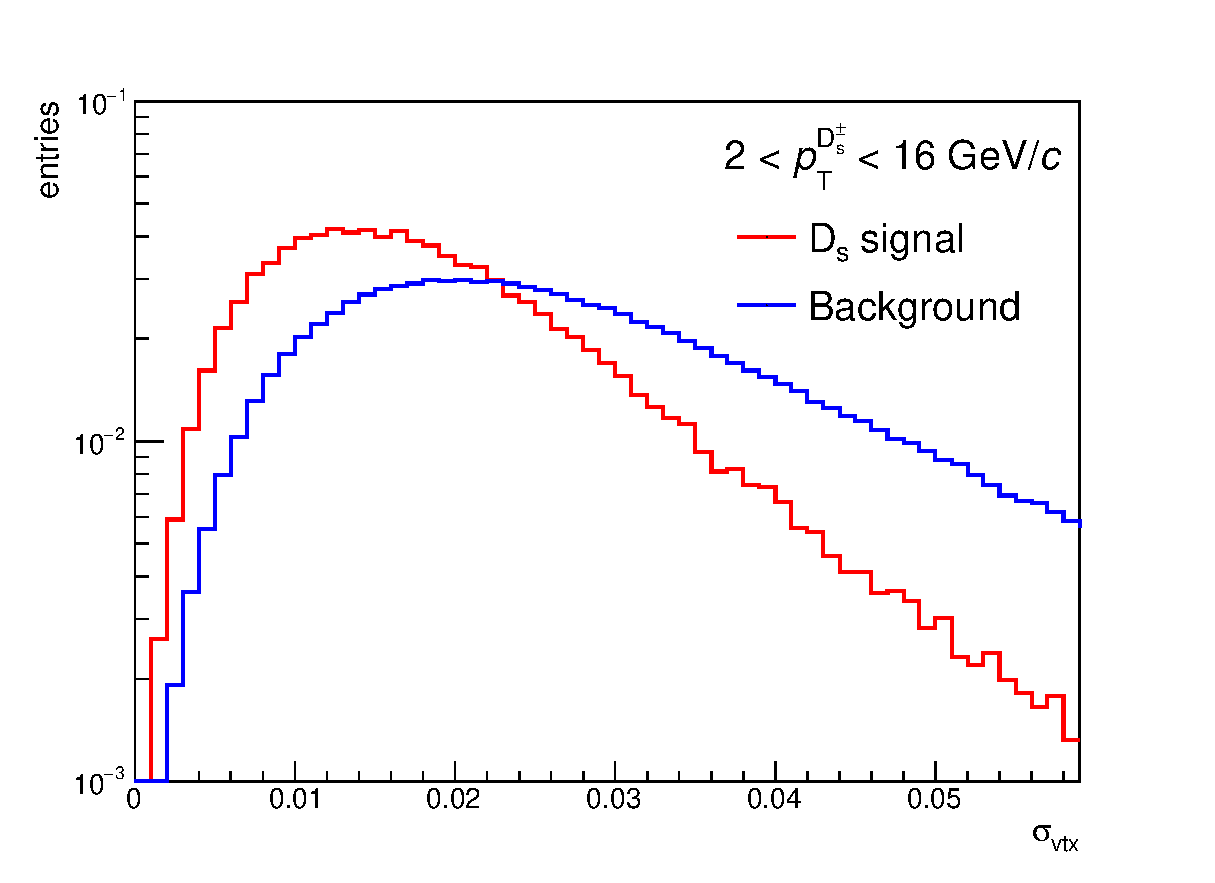
\includegraphics[width=6.5cm]{FigCap4/sigVert.eps}
\caption{Distributions of cos$\theta_{point}$ (left) and track dispersion around secondary vertex $\sigma_{vertex}$ (right) for signal (red) and background (blue) $\Ds$ candidates.}
\label{fig:var2}
\end{figure}
\begin{figure}[!h]
\centering
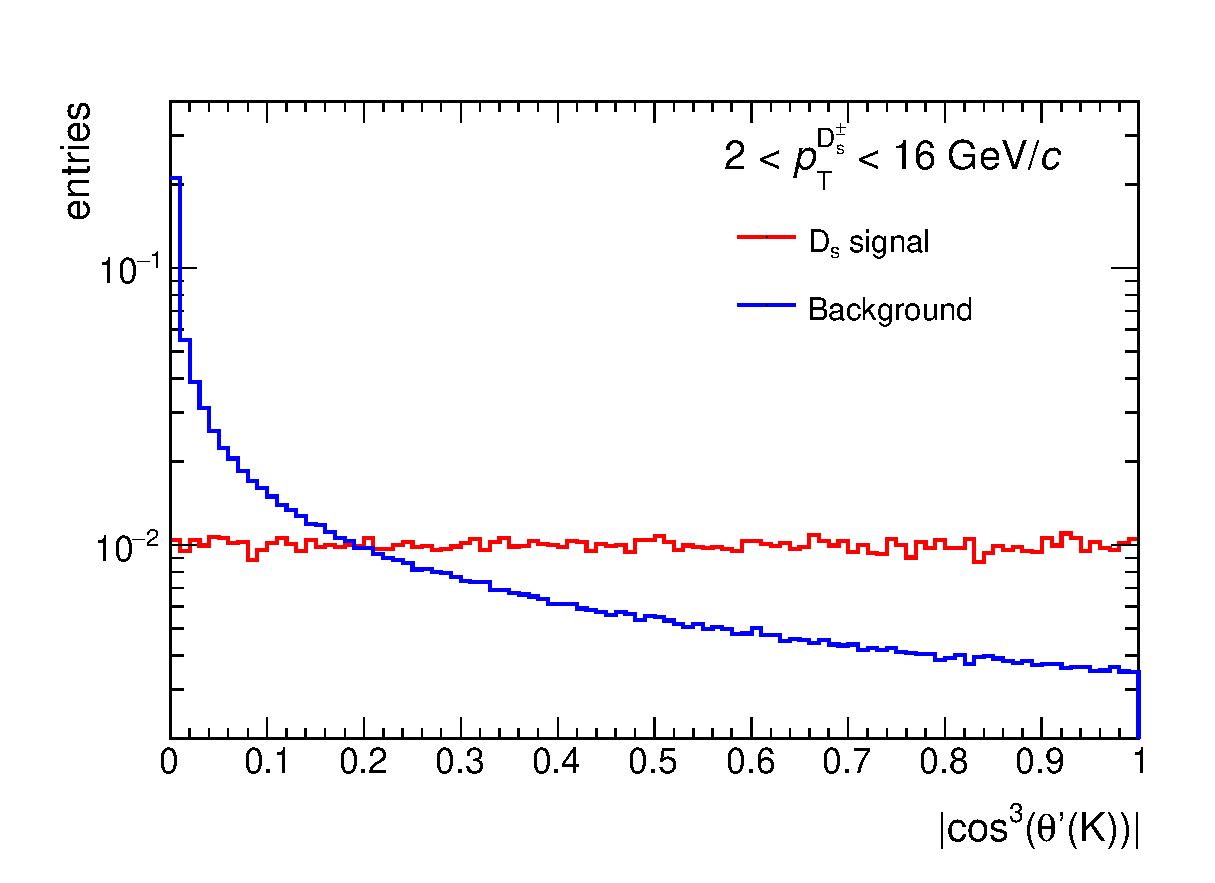
\includegraphics[width=6.5cm]{FigCap4/CosPiKPhi3.eps}
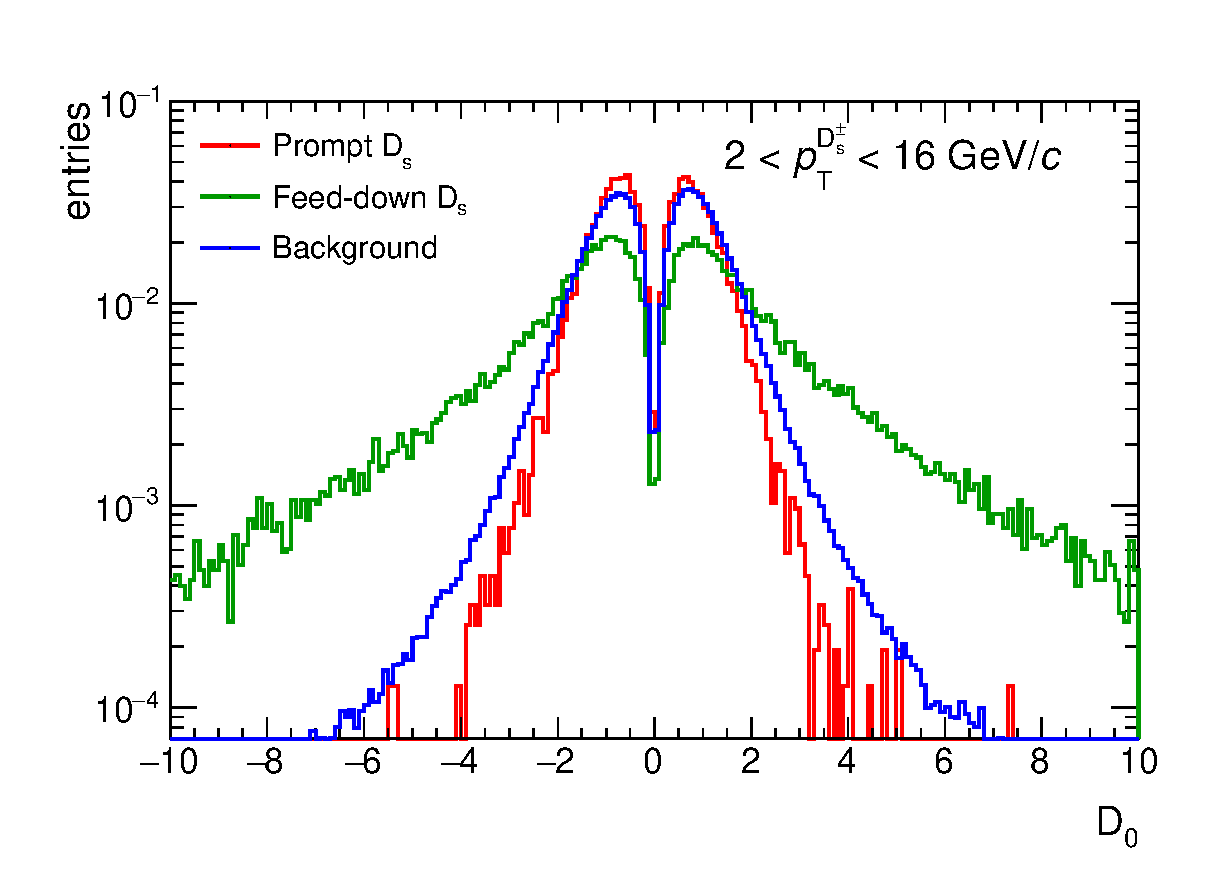
\includegraphics[width=6.5cm]{FigCap4/normIP.eps}
\caption{Left: distributions of $|cos^3(\theta'(K))|$ for signal (red) and background (blue) $\Ds$ candidates. Right: distributions of normalised decay length in the transverse plane for prompt (red), feed-down (green) signal and background (blue) $\Ds$ candidates.}
\label{fig:var3}
\end{figure}

\item \textbf{Track dispersion $\sigma_{vertex}$} around the decay vertex, defined as:
\[
\sigma_{vertex}=\sqrt{d^2_1+d^2_2+d^2_3}
\]
where $d_i$ is the distance of minimal approach between the decay 
track \textit{i} and the decay vertex. All tracks should originate from 
the secondary vertex, and $\sigma_{vertex}$ should be $\sim$ 0; in 
real cases, as a consequence of the tracking and vertexing resolution, 
the $\sigma_{vertex}$ has non-zero values and an upper cut is needed 
to exclude vertices made of random combination of tracks. Typical cut
 values on the track dispersion were between 0.02 $< \sigma_{vertex}<$ 0.05 cm 
 (see Fig.~\ref{fig:var2} right).
\item \textbf{$\theta^*(\pi)$ angle}, it is the angle between the pion 
in the KK$\pi$ rest frame and the KK$\pi$ flight line. Cuts were applied
 on the distribution of the cos$\theta^*(\pi)$, with typical values 
 between 0.95 $<cos\theta^*(\pi)  <$ 1.0.
\item \textbf{$\theta'$(K) angle}, it is defined as the angle between
 one of the kaons and the pion in the KK rest frame. Cuts were 
 applied on the distribution of the $|cos^3(\theta'(K))|$ (Fig.~\ref{fig:var3}, left), with typical 
 values between 0.0 $<|cos^3(\theta'(K))| <$ 0.05.
\item \textbf{Single-track normalised impact parameter residual $IP$} : it is defined 
as the difference between the expected 
impact parameter value $d^{exp}_{0,r,\phi} \approx L_{xy} \cdot sin(\theta_{xy})$
 ($L_{xy}$ is the decay length on $xy$ plane and $\theta_{xy}$ is the angle 
between the reconstructed D meson and the $i$-th daughter track on $xy$ plane) 
and the reconstructed one $d^{reco}_{0,r,\phi}$ for the $i$-th daughter
track, then normalised by the square 
root of their respective uncertainties summed in quadrature. 
In Fig.~\ref{fig:var3} (right) the distributions of the maximum $IP$ among 
daughter tracks of a $\Ds$ candidate are shown, in different colours for
background and true candidates, further distinguished between prompt and beauty 
feed-down components. Since the distributions of the normalised $IP$ residuals 
are quite different for prompt and feed-down D mesons and background candidates, 
a selection based on this variable can reduce the feed-down D-meson efficiency while keeping 
higher that of prompt D mesons. In this analysis selections on the single-track $IP \sim 2$
were applied.
\end{itemize}

The selections on $\theta^*(\pi)$ and $\theta'$(K) angles have already 
been used in various experiments which measured $\Dsplus$ production 
like ZEUS \cite{Chekanov:2005mm} and ATLAS \cite{ATLAS:2011fea} as well as 
in previous ALICE analyses~\cite{ALICE:2011aa,Abelev:2012tca,Adam:2016ich,Adam:2015jda}
 and are based on kinematical 
considerations on the decay chain with a $\phi$ in the intermediate state.
Further selections were applied on the projections of the decay length, 
the normalized decay length and the cos$\theta_{point}$ in the transverse 
plane $xy$. The projections of the variables in the $xy$ plane are instead justified by 
the improving of the impact parameter resolution with respect to $z$-direction.\\


A further parameter which allowed to reduce the background is the
 \textbf{invariant mass of the reconstructed $K^+K^-$ pair}. This is not a topological 
 cut (i.e. a cut exploiting the displacement of the decay vertex), 
 but rather a selection on the decay chain. It is required that at least 
 one of the two pairs of tracks with opposite charge has an invariant
  mass compatible with the $\phi$ mass. The selection is done on 
  the absolute value of the difference between the $\phi$ 
   invariant mass from PDG and the reconstructed one:
\[
\Delta M = |M^{inv}_{rec}-M_{\phi}|.
\]
Typical values for cuts on $\Delta M$ are between 3 $<\Delta M<$ 15 MeV$/c^2$.

\section{Particle identification}
\label{Sec:PID}
The Particle IDentification (PID) selection is based on the specific energy loss 
d$E$/d$x$ in the TPC and the time-of-flight from the interaction vertex to the 
TOF detector. This is used in the D-meson analysis to reduce the background, 
but it is essential for $\Dsplus$ studies because of signal-over-background
 ratios (S/B) of the order of a few percent.
A track is  considered compatible with a certain particle species 
($\pi$, K or p) if the difference between the measured signal is
 within $n\sigma$ from the expected one for the various mass hypotheses
  with the theoretical predictions:
\[
|S_{meas}-S^{\pi,k,p}_{expected}| < n^{\pi,k,p}\sigma ,
\]
where $\sigma$ is the RMS of the Gaussian fit of the theoretical 
curve to the energy-loss or time-of-flight signals for each species.
Candidate triplets were required to have two tracks compatible with 
the kaon hypothesis and one with the pion hypothesis. In addition, 
since the decay particle with opposite charge sign has to be a kaon, 
a triplet was rejected if the opposite-sign track was not compatible 
with the kaon hypothesis. 
The criterion used to combine PID information regarding a track from TPC and TOF
detectors is illustrated in Fig.~\ref{fig:strongPID}, where $n\sigma^{\rm max,TPC} = 1$ for
$0.6 < \pt < 0.8 \, \Gevc$ and 2 elsewhere and $n\sigma^{\rm max,TOF} = 3$ at all $\pt$.  
An output value is associated to the track based on its PID signal in the single
detector: +1 if the track
satisfies $n\sigma^{\rm max}$ selection criteria, 0 if the track satisfies looser selection criteria,
-1 if it is rejected. The responses in TPC and TOF (green values in Fig.~\ref{fig:strongPID}) 
are summed linearly together 
and the track is considered
compatible with the species hypothesis is the final value is 1 or 2. This
PID selection preserves $\sim$85-90\% of the signal depending on the $\pt$.

 
\begin{figure}[!h]
\centering
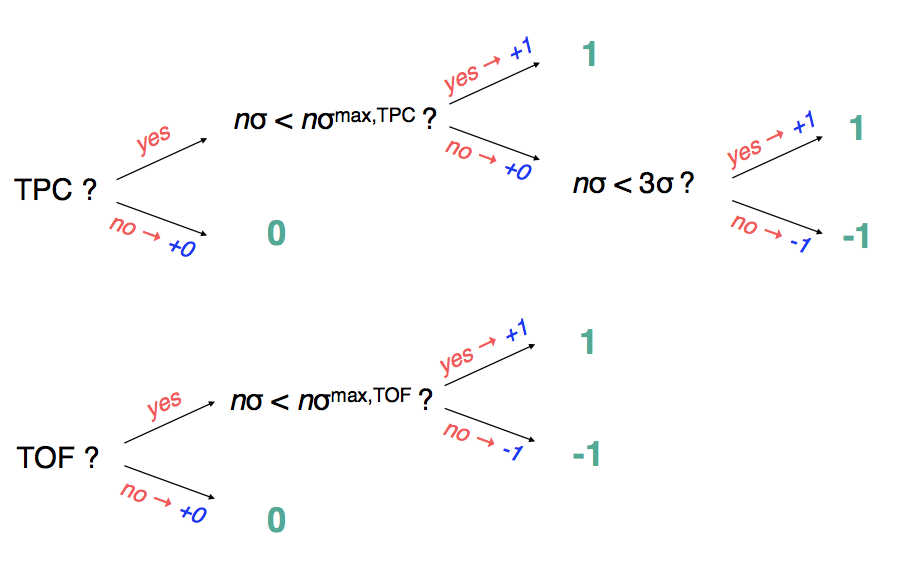
\includegraphics[width=9cm]{FigCap4/strongPID.png}
\caption{PID selection criteria in TPC and TOF for a specific mass hypothesis.}
\label{fig:strongPID}
\end{figure}


\section{Invariant mass spectra and signal extraction}
For each candidate, two values of invariant mass can be computed, 
corresponding to the two possible assignments of the kaon and the 
pion mass to the two same-sign track. In fact, considering the $\Dsplus$
 decay, the charge configuration of the tracks (+, -, +) can be interpreted
  both as to ($K^+,K^-,\pi^+$) and ($\pi^+,K^-,K^+$). Signal candidates with 
  wrong mass assignement to the same-sign tracks would give rise to 
  a contribution to the invariant mass distributions that could introduce
   a bias in the raw yield of $\Dsplus$ mesons. It was verified, both in 
   data and in simulations, that this contribution is reduced to a negligible 
   level by particle identification selection and by the requirement that the
    invariant mass of the two tracks identified as kaons is compatible with 
    the $\phi$ PDG mass.

Once that $\Dsplus$ candidates pass the selections they are 
used to fill invariant mass histograms in different $\pt$ intervals.
The histograms are fitted by a function consisting of a sum of 
a Gaussian and an exponential function to describe the signal peak and 
the background shape respectively:
\begin{equation}
f(x)= Ae^{-B\cdot x}+Ce^{-\frac{(x-\mu)^2}{2\sigma^2}}.
\end{equation}
The selected criterion for the yield extraction was a particle selection 
 strategy that has high efficiency and high statistical 
 significance for the D meson signal, defined as:
\[
Signif = \frac{S}{\sqrt{S+B}},
\]
where S and B are the extracted signal and background obtained 
from the fit procedure integrated within 3$\sigma$ 
around the peak of the Gaussian shape ($\sigma$ being the
RMS of the peak from the fit). The statistical significance is related to the 
relative statistical uncertainty on the extracted signal, so higher 
significance means lower statistical uncertainty on the raw yield. 
A second variable which is used in the cut optimisation procedure
 is the signal-over-background ratio S/B, as 
 an estimator of the powerfulness of the selection strategy. 
 The maximisation of the significance was required together
  with the request that the position of the peak and the width 
  of the Gaussian shape were compatible with the values
   obtained in simulated events, with the same selection strategy.
Since the topological variables have a certain degree of correlation among them, 
for each $\pt$ interval, different parameters 
were simultaneously varied in wide ranges to consider all possible combinations. 
The selection values depend on the $\pt$ of the D-meson candidate and 
are detailed in Table~\ref{tab:cutsDs}.
\begin{table}[tbh!]
\centering
\begin{tabular}{|l|c|c|c|c|} 
\hline 
 $\Ds$ meson& \multicolumn{4}{c|}{pt interval (GeV/$c$)}\\
\hline
 & 2--4  & 4--6 & 6--8 & 8--12\\
\hline
Decay length ($\mum$)        & $>$300 & $>$350 & $>$350 & $>$400\\
Decay length XY ($\mum$)     & $>$0 & $>$200 & $>$200 & $>$200\\
Norm Decay length XY          & $>$2.0& $>$0.0 & $>$2.0 & $>$2.0\\
Cosine pointing              & $>$0.94 & $>$0.95 & $>$0.95 & $>$0.97\\
$\sigma_{vertex}$  (cm)          & $<$0.02 & $<$0.03 & $<$0.03 & $<$0.06\\
M$^{\phi}_{inv}$ - M$^{\phi PDG}_{inv}$ (MeV/$c^{2}$) & $<$8.0 & $<$10.0 & $<$4.5 & $<$9.0\\
$\cos \theta^*(\pi)$    & $<$1.0 & $<$1.0 & $<$1.0 & $<$0.95\\
$|\cos^3 \theta^\prime({\rm K})|$        & $>$0.10 & $>$0.05 & $>$0.05 & $>$0.05\\
Norm. IP residual Kaon  & $<$2.5 & $<$2.0 & $<$2.0 & $<$2.0 \\
Norm. IP residual Pion  & $<$2.5 & $<$2.0 & $<$2.0 & $<$2.0 \\[1ex]
\hline
\end{tabular}
\caption{Selections used for the $\Dspm$ meson in the four transverse momentum intervals considered.} 
\label{tab:cutsDs}
\end{table}
In Fig.~\ref{fig:invmassDs} the invariant mass distributions 
of $\Ds$ mesons in four $\pt$ intervals from 2 to 12 $\Gevc$ are shown.
\begin{figure}[!htb]
\begin{center}
 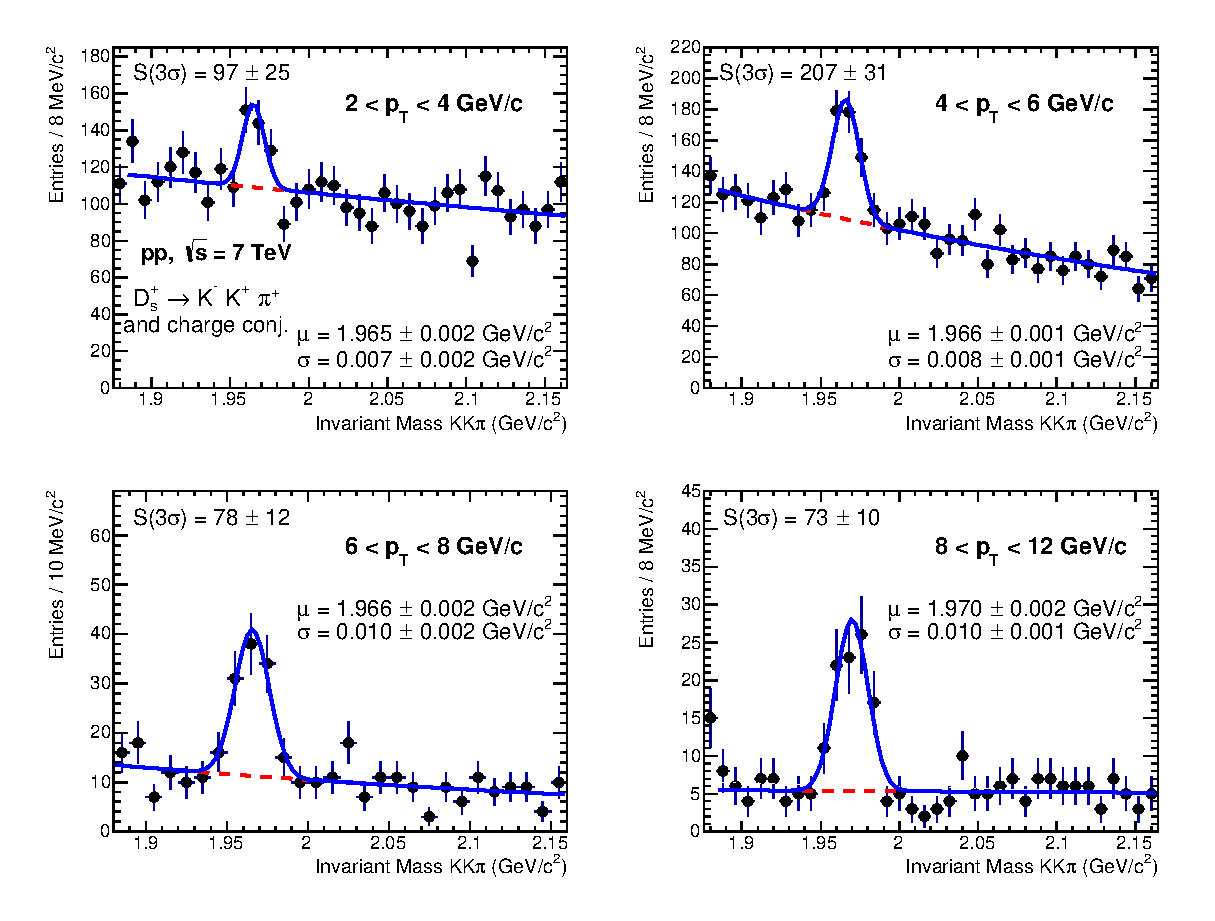
\includegraphics[width=.99\textwidth]{FigCap4/DsMassHistos_ppPass4.eps}
\caption{Invariant mass distributions of $\Dspm$ candidates and charge
conjugates in the four considered $\pt$ intervals.}             
\label{fig:invmassDs}
\end{center}
\end{figure}
An indication of the improved resolution provided by the new 
reconstruction of the sample is shown in Fig.~\ref{fig:sigma4vs2}, where the 
Gaussian sigmas of the invariant mass fits are shown in comparison to 
results of the previous reconstruction, for both data and MC. 
\begin{figure}[!hb]
\begin{center}
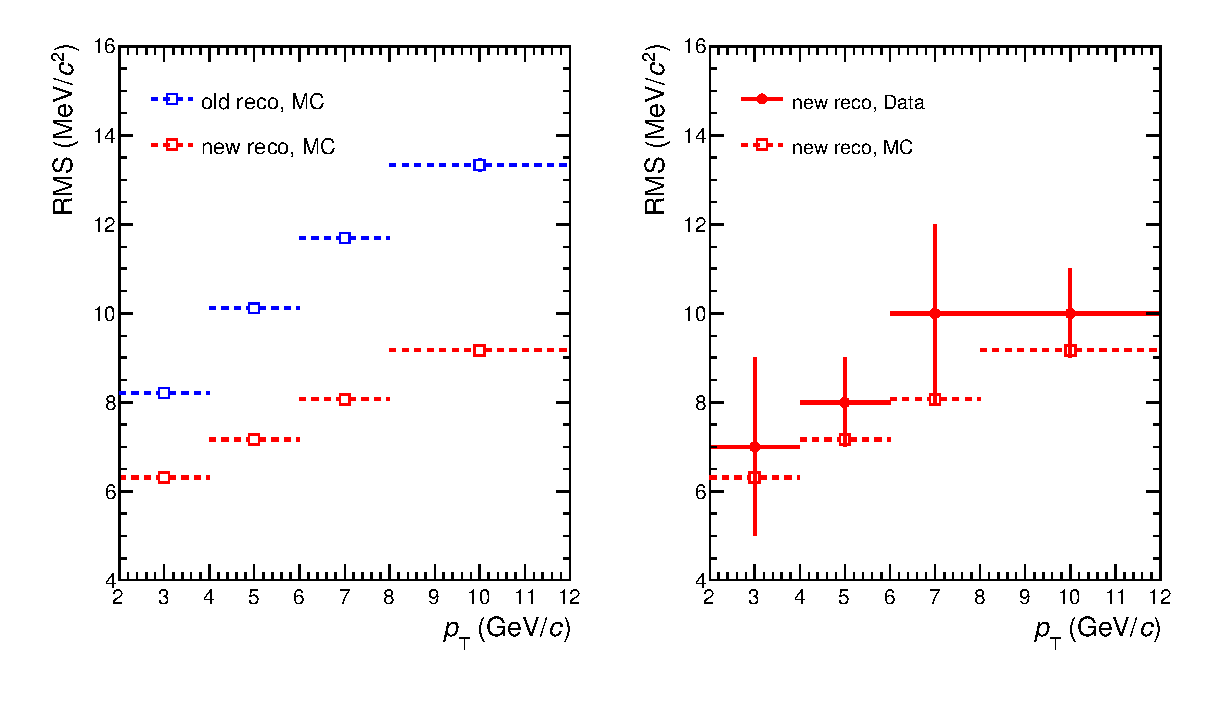
\includegraphics[width=.48\textwidth]{FigCap4/Resolutions_pass2_pass4.eps}
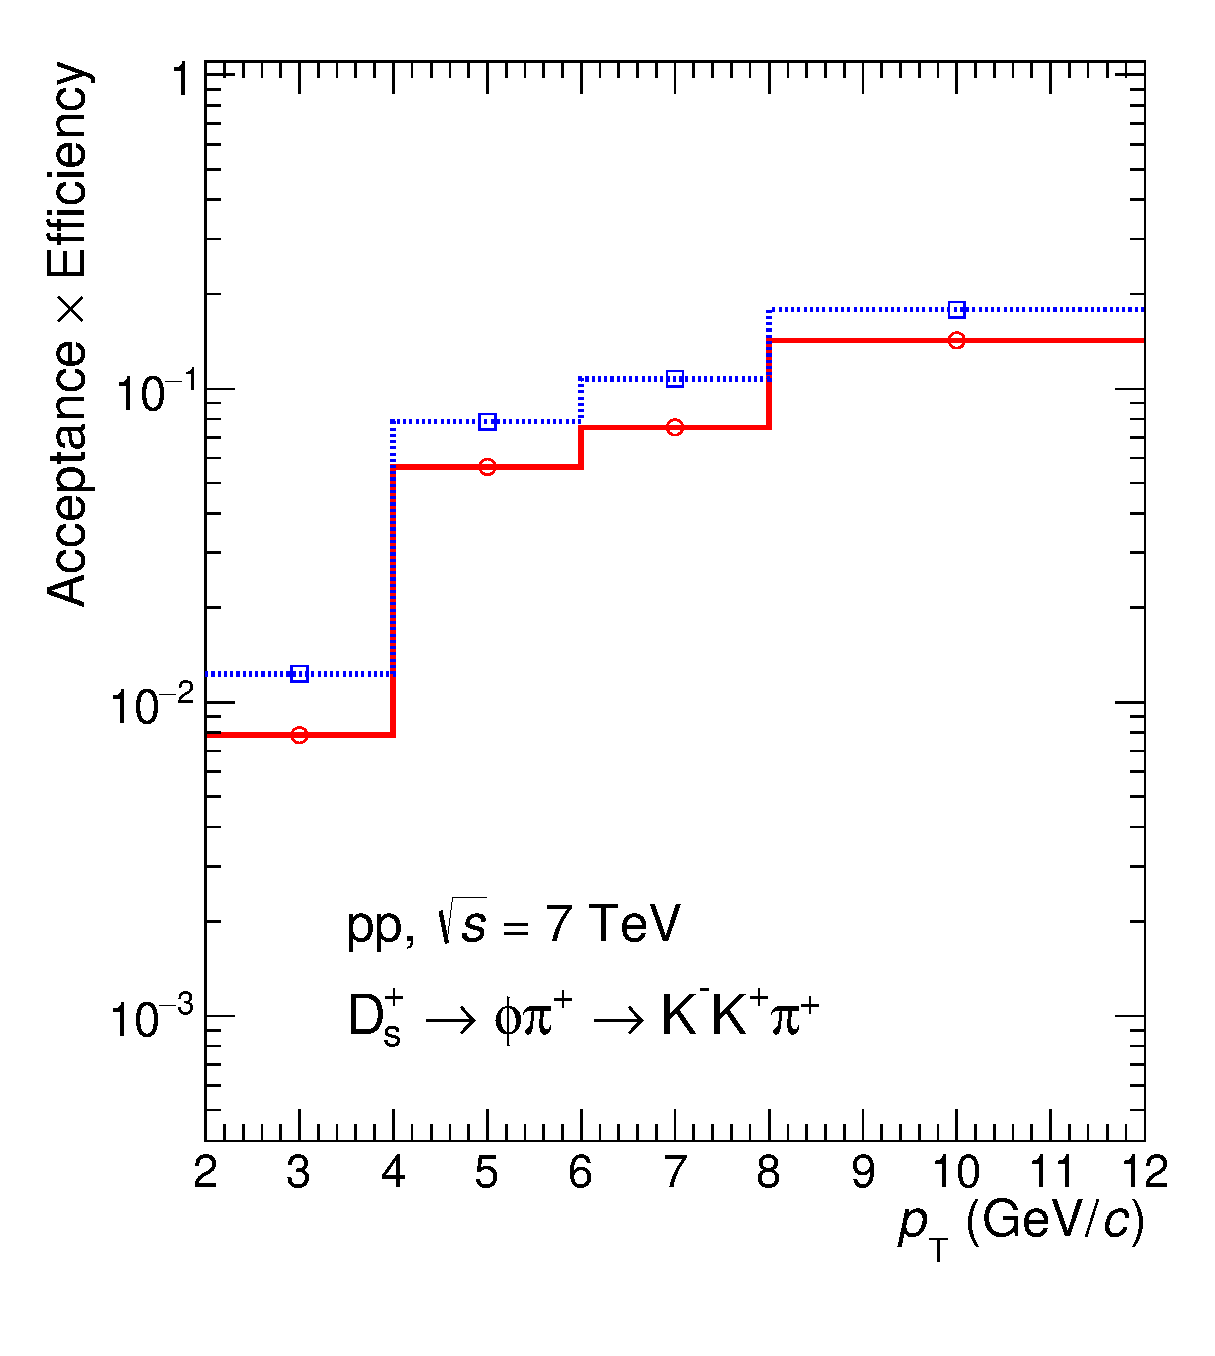
\includegraphics[width=.48\textwidth]{FigCap4/AccEff_Ds_Pass4.eps}
\caption{Left: Gaussian widths of $\Ds$ peak as a function of $\pt$, for current (red) and previous (blue) reconstruction, in data (solid) and MC (dashed). Right: acceptance-times-efficiency of prompt and feed-down $\Ds$ mesons.}
\label{fig:sigma4vs2}
\end{center}
\end{figure}

\section{Corrections}

The $\Dspm$ raw yields extracted from the fits to the invariant-mass distributions
were corrected to obtain the $\pt$-differential production cross sections of prompt
 D mesons. The production cross section was calculated as:
\begin{equation}
  \label{eq:dsdpt}
  \left.\frac{{\rm d} \sigma^{\rm D^{+}_{\rm s}}}{{\rm d}\pt}\right|_{|y|<0.5}=
  \frac{1}{ \Delta \pt}\frac{1}{{\rm BR} \cdot L_{\rm int}}\frac{\left.f_{\rm prompt}(\pt)\cdot \frac{1}{2} N^{\rm D^\pm_{\rm s}~raw}(\pt)\right|_{|y|<y_{\rm fid}}}{ 2 y_{\rm fid}(\pt) \,({\rm Acc}\times\epsilon)_{\rm prompt}(\pt)}\,,
\end{equation}
where $N^{\rm D^\pm_{\rm s}~raw}(\pt)$ is the value of the raw yield 
(sum of particles and antiparticles),
 which need to be corrected for the B-meson decay feed-down contribution 
(i.e.\ multiplied by the prompt fraction $f_{\rm{prompt}}$), divided by the 
acceptance-times-efficiency for prompt $\Ds$ mesons 
$(\rm Acc \times \epsilon)_{\rm{prompt}}$, and divided by a factor of two to 
obtain the charge (particle and antiparticle) averaged yields.
The corrected yields were further divided by the decay channel branching ratio (BR), 
the $\pt$ interval width ($\Delta \pt$), the rapidity coverage 
($2 y_{\rm fid}$) and the integrated luminosity $L_{\rm int}$.
The integrated luminosity was computed as $L_{\rm int} = N_{ev}/\sigma_{pp,MB}$,
where $N_{ev}$ is the number of analysed events and 
$\sigma_{pp,MB} = 62.2$ mb~\cite{Abelev:2012sea}
is the cross-section for the minimum-bias trigger condition, derived from
a Van-der-Meer scan measurement.

\subsection{Reconstruction and selection efficiency}
The acceptance-times-efficiency correction factor, 
$(\rm Acc \times \epsilon)$, was determined for the $\Ds$-meson
hadronic decay considered in this analysis using Monte Carlo simulations 
of pp collisions generated with the PYTHIA 6.4.21 event generator~\cite{Sjostrand:2006za} with the 
Perugia-0 tune~\cite{Skands:2010ak} and particle transport through the apparatus 
using GEANT3~\cite{Brun:1994aa}.
The luminous region distribution and the conditions (active channels, gain, 
noise level and alignment) of all the ALICE detectors were included in the 
simulations, considering also their evolution over time during the 2010 LHC 
data taking period.
In the production, only events containing a $c\bar{c}$ or a $b\bar{b}$ pair 
were transported through the apparatus and reconstructed and
D mesons were forced to decay hadronically via the decay channel relevant to
the specific analysis.
The efficiency was extracted separately for prompt and feed-down D-meson and 
is shown in the right panel of Fig.~\ref{fig:sigma4vs2}.
D mesons from beauty decay have higher efficiency than
the prompt ones in all the $\pt$ intervals, due to the more displaced 
decay vertex from interaction point.
In general, with the chosen topological selections, efficiencies in this analysis
are on average 15\% lower than those used in the previous reconstruction. 
The present analysis uses more powerful selection variables 
(projections on $xy$ plane and impact parameter residual) that
enhance the signal-over-background ratio for $\Ds$ meson by a factor 
from 2 to 5 depending on the $\pt$ interval, with an acceptable worsening
of the global efficiency. Large signal-over-background ratios are indeed essential 
to assure a good stability of the extracted yield.

\subsection{B-feeddown subtraction}

The $f_{\rm prompt}$ fraction was calculated using the beauty production cross sections from  
FONLL calculations~\cite{Cacciari:1998it, Cacciari:2001td}, the 
$\mathrm{B} \rightarrow \mathrm{D} + X$ decay kinematics from the EvtGen package~\cite{Lange:2001uf} 
and the efficiencies for feed-down D mesons reported in 
Fig.~\ref{fig:sigma4vs2} (right):
\begin{equation}
\label{eq:fpr}
f_{\mathrm{prompt}} =1- \frac{N^{\text{D~feed-down}}_{\mathrm{raw}}}{N^{\mathrm{D}}_{\mathrm{raw}}}= 1- \left (\frac{\rm d^2 \sigma}{\mathrm d\pt \mathrm d y} \right)^{\rm FONLL}_{\text{feed-down}} \cdot \frac{(\mathrm{Acc} \times \epsilon)_\text{feed-down} \cdot \Delta y \Delta \pt \cdot \mathrm{BR} \cdot L_{\rm int}}{N^{\rm D +\overline{D},raw}/2}\,,
\end{equation}
where the $\pt$ dependence of $f_{\rm prompt}$, $N^{\rm D +\overline{D},raw}$ and
$(\mathrm{Acc} \times \epsilon)_\text{feed-down}$ is omitted for brevity.
The values of $f_{\rm prompt}$ of $\Ds$ meson are shown in Fig.~\ref{fig:fprompt} as a function of $\pt$.
\begin{figure}[!hb]
\begin{center}
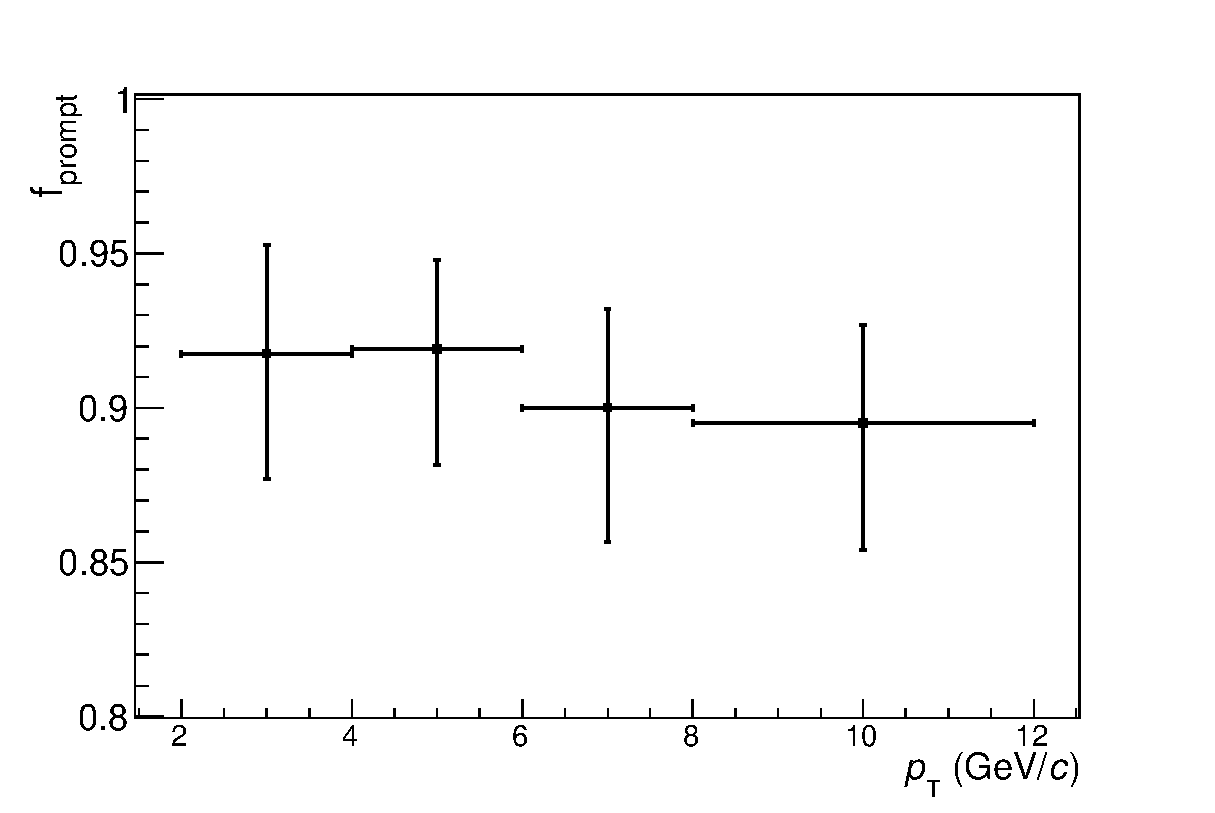
\includegraphics[width=.48\textwidth]{FigCap4/promptFraction_pass4.eps}
\caption{Prompt fraction values for $\Ds$ meson with the final selections as a function of $\pt$ in pp collisions at $\s = 7$ TeV.}
\label{fig:fprompt}
\end{center}
\end{figure}



\section{Systematic uncertainties}
In this section the study of the systematic uncertainties for the
 measurement of the $\Dsplus$ cross section as a function of $\pt$ is presented. 
 The contributions to the systematic uncertainty from different 
 sources were studied separately and described in detail in the following.

\subsection{Raw yield extraction}
Systematics on the yield extraction were evaluated by studying 
the variation of the raw yields in each $\pt$ interval when 
varying the line shape for the signal and the fitting function for the 
background. Let's examine these two contributions separately.\\



\emph{Signal line shape}
The uncertainty from signal line shape was calculated by 
considering the combinations among these fit
configurations: (i) free Gaussian width parameter, (ii) free mean parameter, 
(iii) width parameter varied by 20\% with respect to MC value, (iv) width parameter 
fixed to MC value, (v) mean parameter fixed to MC value.
The error was extracted as the maximum error ((max. value - min. value)/2) divided by square root of 12.
It resulted in a 5\% systematic uncertainty in all the $\pt$ intervals.

\emph{Background fit function}
Using different functions to fit the background could in 
principle introduce some systematic difference in the extracted yields.
The default shape used to give the central yield is an 
exponential function, but first and second 
order polynomial shapes were also tested. In Table~\ref{tab:chi2bkg} 
the values of reduced chi square referred to the compatibility 
of the background function with data (excluding peak region) are 
reported. One can see that all the three shapes 
give a good description of data, but in general no improvements 
are visible when adding more parameters in the fit
with respect to exponential shape, so the latter confirms itself as a good choice.
Neverthless, it is important to look also at the values of the 
extracted yield to assess about possible biases.
 In order to do this, 50 simulated samples were generated via 
 Poissonian smearing of the fit function with the exponential background.
 For each sample, yields extracted with exponential 
 background were compared with those using linear and 
 polynomial functions with the same
configuration for pole, sigma, mass range and bin width, and their
difference, normalised to the yield with exponential background, 
used to fill a histogram. The procedure was repeated for different
configurations of pole, sigma, mass range and bin width. 
A potential shift from zero of the mean of the resultant distribution 
 should reveal the bias from the change of background. The
  spread of the distribution is related to statistical fluctuations. 
  In the top panels of Fig.~\ref{fig:diffBkgPt0} an example of the above 
  described distribution is presented, in the interval $2 < \pt < 4\, \Gevc$.
  The left and right panels shows respectively the distribution of the difference
  of yields extracted with linear or Pol2 shapes to those extracted with exponential
  background. The shift in the distribution is not statistically significant 
 since $\mu < 3\sigma$.
 \\
The systematic from the yield extraction is hence a 5\%. 
It results reduced by a factor 3-4 with respect to the analysis of pass2,
where it was around 15-20\% depending on the $\pt$ interval. 

\begin{table}[!t]
\centering
\vspace{0.5cm}
\begin{tabular}{|c|c|c|c|c|} 
\hline \rule{0pt}{2.7ex}
 & $\pt$ interval & Exponential & Linear & Pol2 \\ 
 &(GeV/$c$) & & &  \\ 
\hline \rule{0pt}{2.7ex}
           &\phantom{0}2--4\phantom{0} & 1.21 & 1.21 & 1.09\\
           $\chi^2/ndf$ &\phantom{0}4--6\phantom{0} & 1.15 & 1.18 & 1.16\\
          &\phantom{0}6--8\phantom{0} & 1.03 & 1.02 & 1.03\\
           &\phantom{0}8--12 & 0.99 & 0.99  & 1.03\\
\hline
\end{tabular}
\caption{Reduced $\chi^2$ values for the fit of the background (peak region excluded) in the
considered $\pt$ intervals of the $\Ds$ meson.} 
\label{tab:chi2bkg}
\end{table}

\begin{figure}[!htb]
\begin{center}
 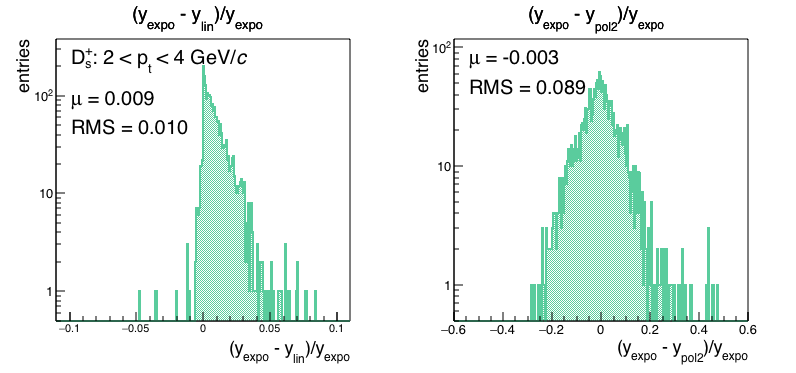
\includegraphics[width=.70\textwidth]{FigCap4/studyBkg_Free_pt0.png}
\caption{Relative difference of signal yield with exponential and linear (left) and Pol2 (right) 
functions for background for $2 < \pt < 4 ~\Gevc$.}             
\label{fig:diffBkgPt0}
\end{center}
\end{figure}


\subsection{Selection efficiency}

The systematics on the selection efficiency accounts for 
possible imperfections in the MC description ($\pt$, 
impact parameter resolution) which could 
impact the raw yield correction via the efficiency term.
A possible test to quantify the effect of imperfections in the 
description of topological variables in the MC is to exploit different sets of cuts
that have different selection efficiencies and to compare the corrected
yields. In this analysis, twelve sets of cuts with 
medium-high statistical significance of the extracted yields were compared, 
their respective efficiencies spanning a variation of
a factor from 2 to 6, depending on the $\pt$ interval. We take the RMS 
of the corrected yield distribution in each $\pt$ interval as an estimator of 
the systematic uncertainty. The uncertainty resulted in a 7\% in all $\pt$ bins.
\begin{figure}[!b]
\begin{center}
 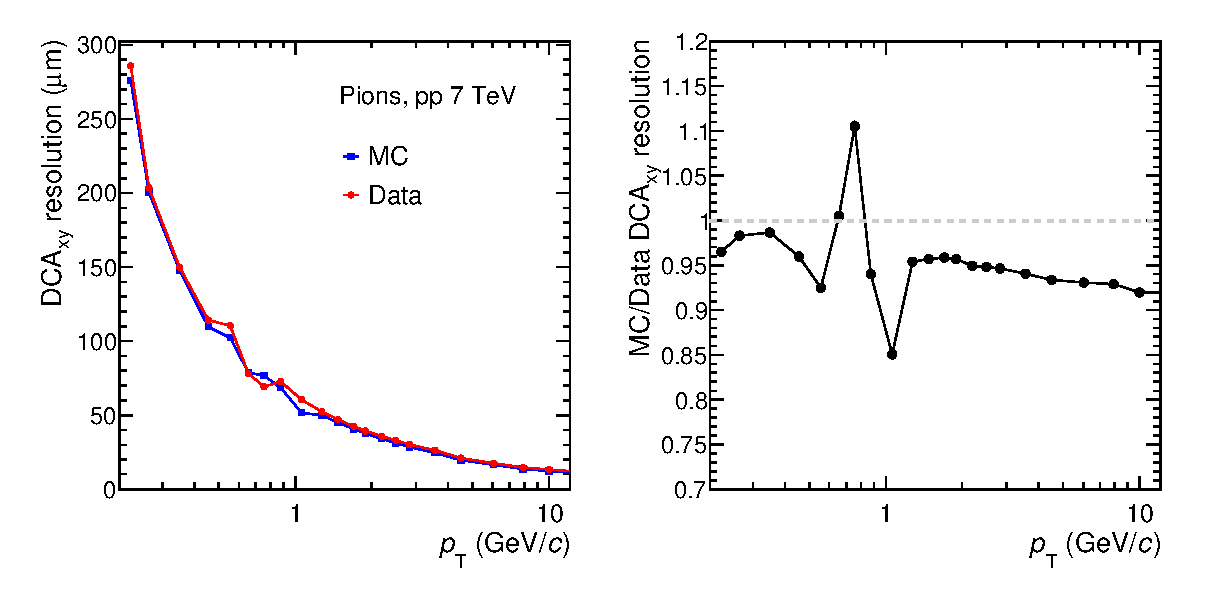
\includegraphics[width=1\textwidth]{FigCap4/DCAxyReso_Pions.eps}
\caption{DCA$_{\rm xy}$ resolution curves of pion tracks as a function of $\pt$ in data and in MC (left panel) and their ratio (right panel) in pp collisions at $\s = 7 $ TeV.}             
\label{fig:DCAxyReso}
\end{center}
\end{figure}
The effect of a variation of the impact parameter resolution in the transverse plane
was also investigated. Fig.~\ref{fig:DCAxyReso} (left) shows, as an example for pion tracks, distributions of
DCA$_{\rm xy}$ resolution as a function of $\pt$ in data and in simulation 
in pp collisions at $\s = 7 $ TeV. The values were extracted via fits to the DCA$_{\rm xy}$ distributions
of tracks in data and in MC, in different $\pt$ intervals, and estimated as the RMS of
such fits. The right panel of the Fig.~\ref{fig:DCAxyReso} shows the ratio MC to data of DCA$_{\rm xy}$ resolutions. 
The agreement is overall good; to estimate the effect of the residual discrepancy at hight $\pt$,
the resolution values in MC were reduced up to 10\% and the
DCA$_{\rm xy}$ of tracks in MC smeared according to the new resolution.
The variation of the efficiencies results in less than 3\%, which is hence
included in the already quoted 7\% from previous discussion. 
\iffalse
\begin{figure}[!htb]
\begin{center}
 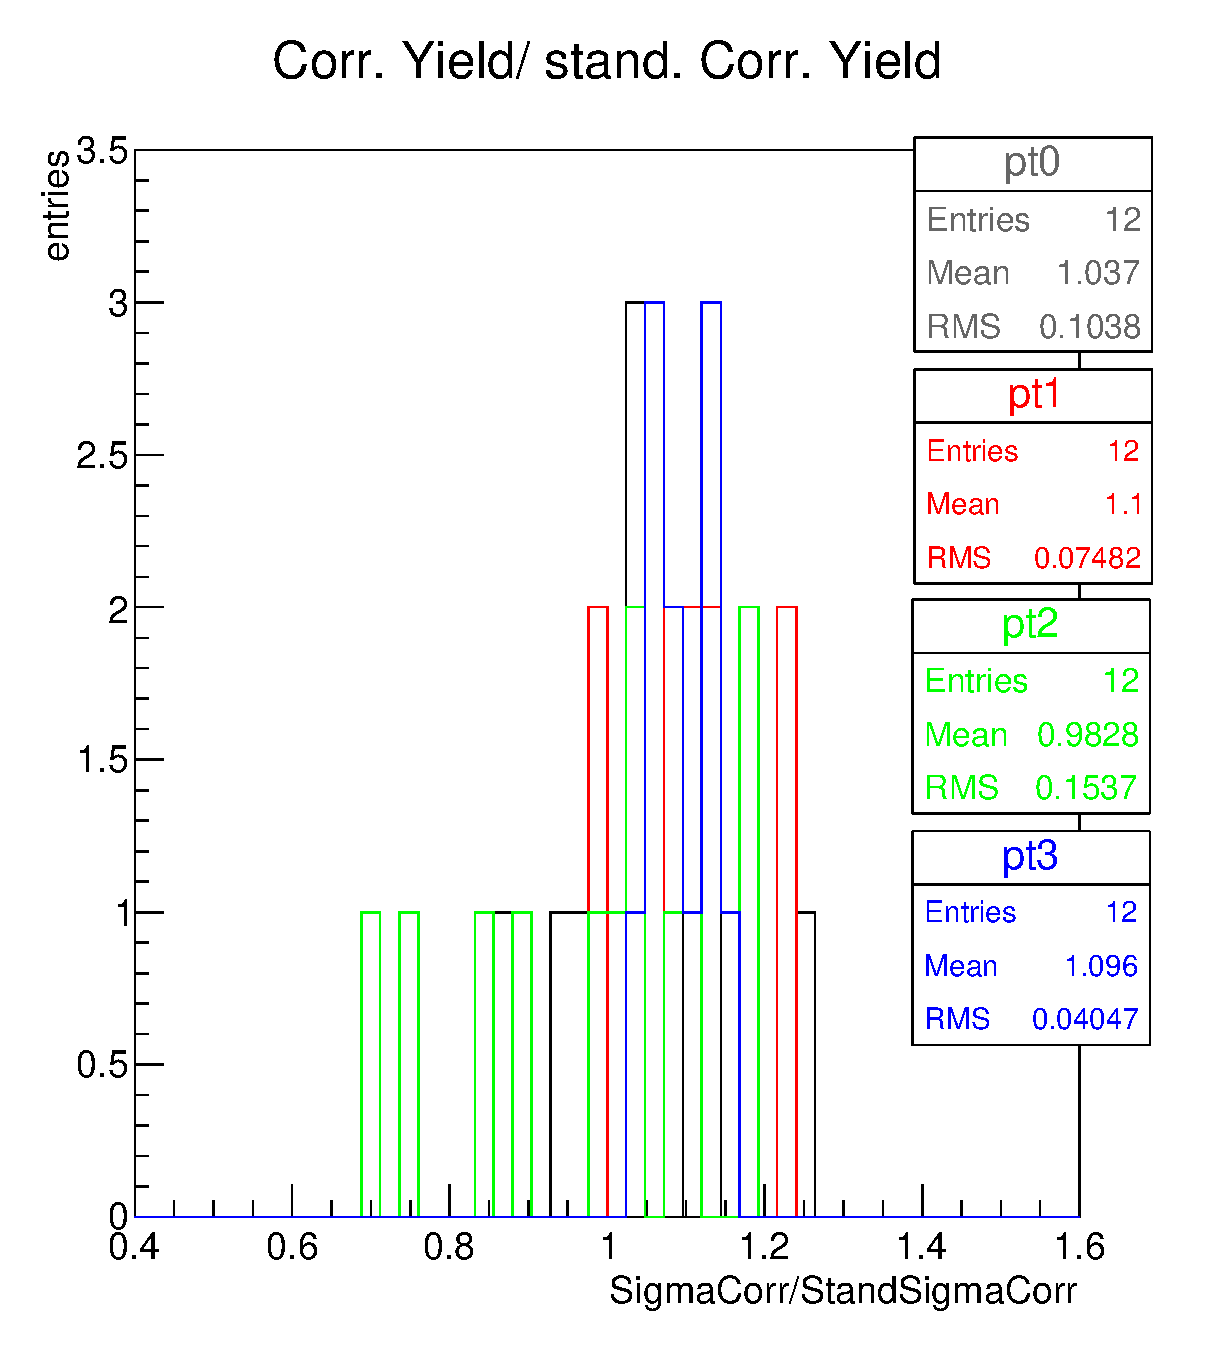
\includegraphics[width=.44\textwidth]{FigCap4/rms_cutvariation.eps}
 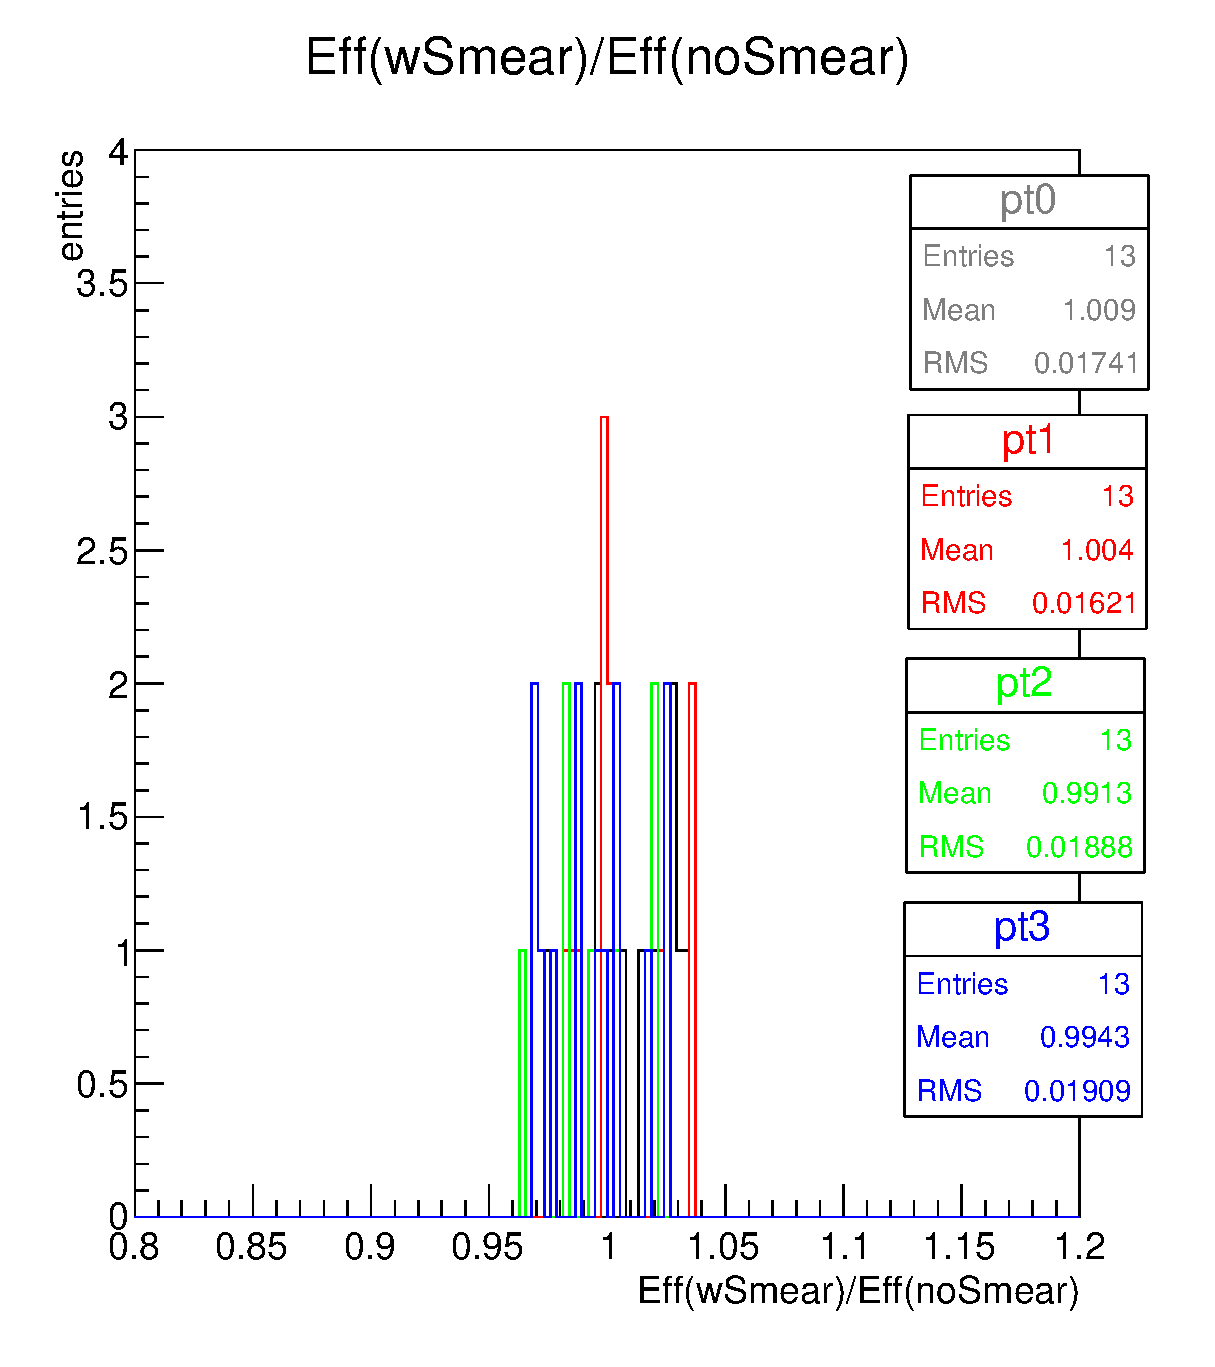
\includegraphics[width=.44\textwidth]{FigCap4/rms_smearp10.eps}
\caption{Left: $\Ds$ corrected yield measured with 12 different sets of
cuts and compared to the yield from the best set of cuts (chosen for the central yield value). Right: ratio for $\Ds$ efficiencies w/o a 
10\% smearing on the xy impact parameter resolution.}             
\label{fig:cutVariation}
\end{center}
\end{figure}
\fi

\subsection{PID efficiency}
To test the efficiency correction of PID selections, a looser PID cut
was used with respect to the default selection described in Sec.~\ref{Sec:PID}. 
In fact, in the $\Ds$ case, the rare signal and the large background 
do not allow for a signal extraction without 
particle identification. This looser PID selection accepts those cases 
reported in Fig.~\ref{fig:strongPID} where combined response value from TPC and TOF 
detectors is $\geqslant 0$.
In Fig.~\ref{fig:rmsPID} the ratio
of the corrected yield obtained with looser to default PID selection is shown, 
for the twelve different sets of cuts discussed before.
The evaluation of the systematic uncertainty, estimated from the RMS of the distributions in each $\pt$ 
interval, was made considering $\pt > 4 \, \Gevc$, since at lower $\pt$ 
the yield extraction with looser PID does not guarantee a statistical significance
of the signal peak larger than 3. The RMS of the yield distributions for the considered
$\pt$ intervals is around 7\%.

\begin{figure}[!htb]
\begin{center}
 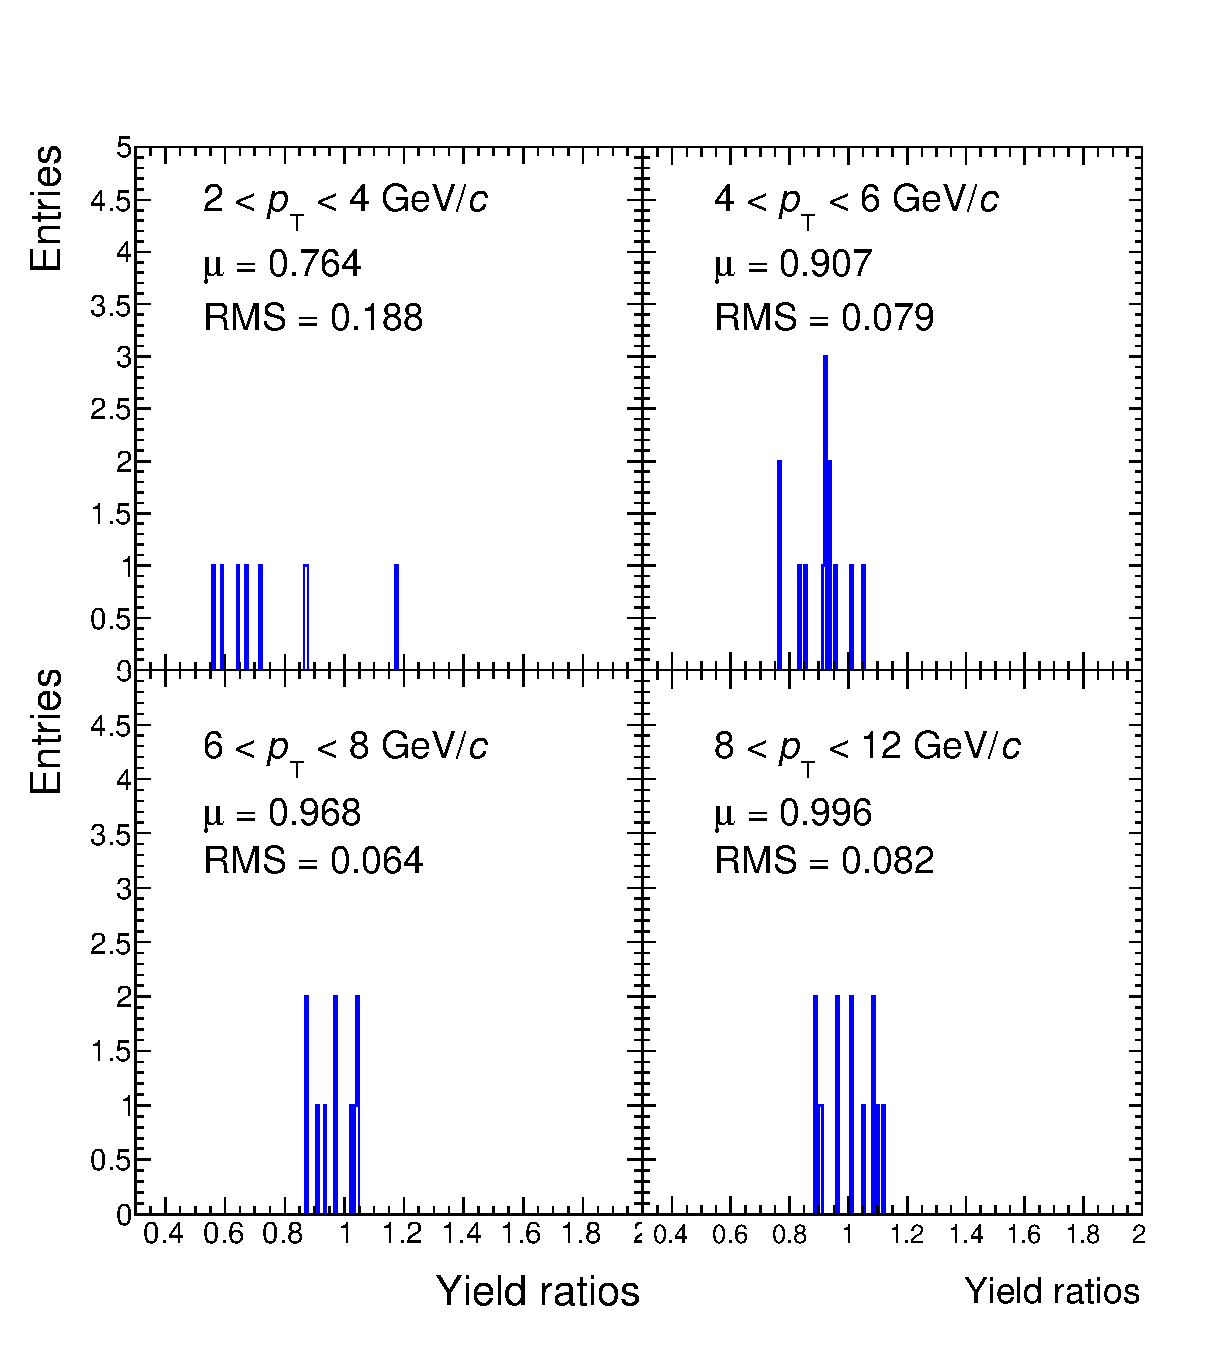
\includegraphics[width=.7\textwidth]{FigCap4/PIDrms4x4}
\caption{Ratio of $\Ds$ corrected yields with looser and default PID selections (twelve different sets of
topological selections).}
\label{fig:rmsPID}
\end{center}
\end{figure}

\subsection{Track reconstruction efficiency}

The systematic uncertainty related to the tracking efficiency includes the 
effects arising from track finding in the TPC, from track prolongation  
from the TPC to the ITS, and from track quality selections.
It was estimated with the following tests:
\begin{itemize}
\item comparison of the D-meson cross sections obtained with different track selection cuts;
\item comparison of the TPC-ITS track matching efficiency in data and simulations.
\end{itemize}
These checks are discussed in detail in the following subsections.

\subsubsection{Variation of track selections}
For this purpose $\Dzero$ and $\Dplus$ mesons were used due to their
higher statistical significance of the extracted yields.
The D-meson raw yields and efficiencies were evaluated with 
different sets of track selection cuts.
The following selections were tested:
\begin{enumerate}
\item additional cut on number TPC crossed rows $> 120-(5/\pt)$;
\item number of TPC clusters $>0.65 \times$ number of TPC crossed rows;
\item ratio of crossed rows over findable clusters in the TPC $>0.9$.
\end{enumerate}
The systematic uncertainty was assigned based on the observed variation of
the prompt $\Dzero$ and $\Dplus$ cross sections with respect to the default selections.
Based on this check a systematic uncertainties of 2\% and 3\% were 
respectively estimated for $\Dzero$ (two-body decay) and $\Dplus$ (three-body decay) 
due to variation of track cuts, which is consistent with a 1\% per-track systematic
uncertainty.

\subsubsection{ITS-TPC matching efficiency}

Matching efficiency is defined as the fraction of tracks with 
clusters in both ITS and TPC over the number of tracks with clusters in TPC.
Systematic uncertainty on its determination arises from discrepancies 
in efficiency between data and Monte Carlo.
Matching efficiency for primary tracks is expected to be higher than 
for secondary tracks (originating from strangeness decay, thus 
with secondary vertices likely to be out of SPD) or tracks arising
 from interaction with material.
If the fractions of primary and secondary tracks are different in data 
and in Monte Carlo, this could lead to a wrong estimation of systematic 
uncertainty in the matching. Hence, the idea of this study is to 
use data-driven corrections of primary and secondary fractions in the MC.
to obtain a corrected inclusive MC efficiency. The latter will be compared 
with efficiency on data to extract the systematic uncertainty.\\
The ingredients are:
\begin{itemize}
\item matching efficiencies for different particle types: 
Eff$^{\rm MC}_{\rm primaries}$, Eff$^{\rm MC}_{\rm secondaries}$, Eff$^{\rm Data}_{\rm inclusive}$
\item fraction of primary tracks in data: f'$_{\rm primaries}$
\item corrected MC-inclusive efficiency: 
Eff$^{\rm MC}_{\rm inclusive}$ = f'$_{\rm primaries}$ x Eff$^{\rm MC}_{\rm primaries}$ + (1- f'$_{\rm primaries}$) x Eff$^{\rm MC}_{\rm secondaries}$
\item systematic uncertainty: 
(Eff$^{\rm Data}_{\rm inclusive}$ - Eff$^{\rm MC}_{\rm inclusive}$)/Eff$^{\rm Data}_{\rm inclusive}$.
\end{itemize}
A minimum-bias Monte Carlo production anchored to 2010 pp data taking at 
$\s = 7$ TeV was used. Charm-enriched productions were not used in this study 
since the shape of DCA distribution of tracks (used to extract data-driven 
primary track fraction) is affected by the heavy-flavour enhancement
and may bias the fit.
Efficiency was studied as a function of:
\begin{itemize}
\item $\pt$, from 0.5 to 15 $\Gevc$
\item $\phi$, between (0,2$\pi$)
\item $\eta$, between (-0.8,0.8)
\end{itemize}

Let's examine below in detail the steps needed to 
calculate the systematic uncertainty.
\begin{enumerate}
\item {\bf ITS-TPC matching efficiency:} calculated separately for 
primary and secondary tracks in MC, inclusively on data. For 
the numerator of the efficiency, tracks were selected requiring 
to have a hit at least in one of the SPD layers, 
$|$DCAxy$|<$ 2.4 cm and $|$DCAz$|<$ 3.2 cm.
\begin{figure}[!htb]
\centering
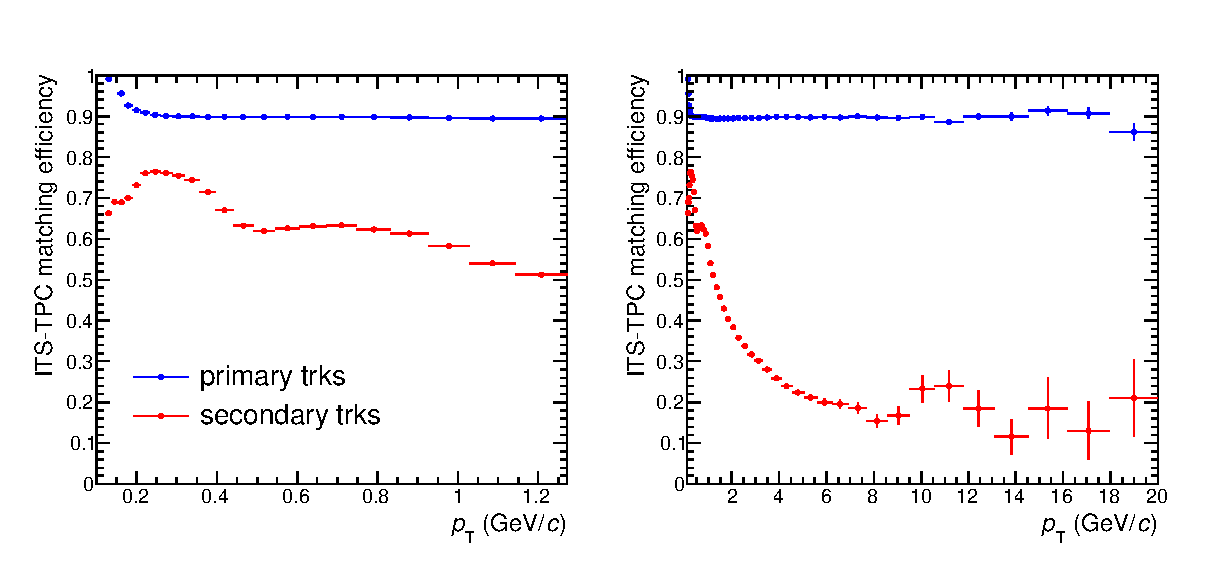
\includegraphics[width=1\textwidth]{FigCap4/ITSTPC_matchEff_vsPt_LowFullpt.eps}
\caption{Matching efficiency for primaries and secondaries tracks as a function of $\pt$ in MC for $\pt$ intervals from 0.1 to 1 $\Gevc$ (left) and from 0.5 to 20 $\Gevc$ (righ). }
\label{fig:matcheff_pt}
\end{figure}

In Fig.~\ref{fig:matcheff_pt}, ITS-TPC matching efficiency 
of charged tracks in MC as a function of 
$\pt$ is shown. The left panel is referred to the low $\pt$ region (0.1-1 $\Gevc$), 
the right one to a wider range from 0.5 to 20 $\Gevc$. 

\item {\bf Fractions of primary tracks:} extracted from a fit to
 the track impact parameter distribution in data using MC templates for 
 DCA distributions of primary and secondary tracks. The ROOT TFractionFitter 
 package was used to perform the fit. The fit could be resolved 
 using three templates describing primary tracks, secondaries tracks
 from strangeness decay and tracks from interaction with material. 
 A selection on tracks requiring at least one hit in the two SPD layers 
 was used, to assure enough resolution to distinguish primary and 
 secondary DCA distributions.
Fit was performed on the DCA$_{\rm xy}$ distributions of charged particles 
in the range [-1,1] cm, in different intervals of $\pt$, $\phi$, $\eta$ 
and constraining the three fractions within reasonable minimum and maximum values.
The fractions were then calculated by integrating the histogram 
resulting from the fit in the range $|$DCA$_{\rm xy}|<$ 2.4 cm, for
consistency with what done for matching efficiency calculation. 
As a closure test, it was verified that the MC fractions of primary and secondary tracks 
were in agreement with the values extracted if performing the fit using TFractionFitter 
on the inclusive MC distribution (instead of data), with the three MC templates.  
In Fig.~\ref{fig:DCAxyDataMCVsPt} the distributions of DCA$_{\rm xy}$ 
in data and in MC for the different contributions are
shown in different colours, in $\pt$ intervals from 0.5 to 15 $\Gevc$. 
In Fig.~\ref{fig:DCAxyRatioDataFitVsPt} the ratio of DCA$_{\rm xy}$ distributions 
of data to the histogram resulting from the fit are plotted. 
Finally, in Fig.~\ref{fig:Fractions}, the data-driven values of primary and secondary
 fractions are shown and compared to 
 the ones obtained from MC truth (empty markers). 
The fraction of secondaries in the figure already includes contribution 
from material. We conclude that the fraction of secondaries is underestimated in MC.

\item {\bf Correction to the primary fraction:} since the fraction of primary
 particles was calculated using tracks with the request of a hit in one of the SPD layers, we
need to rescale the primary fraction to the total number of tracks in TPC. 
The correction factor is based on MC information and obtained as 
the ratio of the fraction of primary tracks in TPC with the fraction of primary
 tracks with match TPC-ITS. The final fraction of primary tracks is hence
  f'$_{\rm primaries}$ = f$_{\rm primaries}$ x correction factor, 
  where f$_{\rm primaries}$ is the fraction obtained at step 2. 
  Typical values of correction factor are around $\sim$ 0.95-0.98. 
  In Fig.~\ref{fig:MCfractions} an example of fractions of primary 
  and secondary tracks in MC requiring ITS-TPC or TPC only are 
  shown in different colours as a function of $\pt$.

\item {\bf ITS-TPC corrected matching efficiency:} calculated 
as  Eff$^{\rm MC}_{\rm inclusive}$ = f'$_{\rm primaries}$ x Eff$^{\rm MC}_{\rm primaries}$ + (1- f'$_{\rm primaries}$) x Eff$^{\rm MC}_{\rm secondaries}$. The corrected matching efficiency 
is shown in Fig.~\ref{fig:CorrMatchEffVsPt},~\ref{fig:CorrMatchEffVsPhi}, 
as a function of $\pt$, $\phi$, $\eta$ respectively, for kaons and 
pions only (using particle identification, requiring a 3-sigma cut). 
It was verified that no substantial changes are obtained if 
considering all the species (pions, kaons, protons, electrons, muons). 
Finally, the ratios of the latter inclusive MC-corrected efficiencies with
 data are shown in Fig.~\ref{fig:SysMatchEffVsPt},~\ref{fig:SysMatchEffVsPhi},~\ref{fig:SysMatchEffVsEta}. 
 It is evident how the re-weighting of MC with the real fractions 
of track types is useful in quoting a truthful and reduced systematic uncertainty. \\ 
Error bars were assigned to matching efficiency to account for statistical fluctuations.
A final systematic uncertainty of 2\% per track is assigned for particles 
between 2-6 $\Gevc$, and of 1\% at lower and higher $\pt$.
This per-track uncertainty needs to be summed in quadrature with the 
1\% uncertainty coming from systematic on track selection. \\
Finally, a MC simulation was used to propagate the uncertainty at the 
track level to the D meson level, accounting for the daughter's 
kinematic in the D-meson $\pt$ range of our analysis. In the MC 
simulation the same topological and PID cuts used on data were 
applied, to account also for possible influence of topological selection
 on daughter's kinematics. In the left column of 
 Fig.?, one can see the 
scatter plot of D-meson $\pt$ versus daughter's $\pt$ 
(for $\Dplus$, $\Ds$ and $\Dzero$ from top to bottom). 
The right column shows instead the final systematic on matching
 efficiency we quote for 2- and 3-prong D mesons as a function of $\pt$.
\end{enumerate}

\begin{figure}[!htb]
\begin{center}
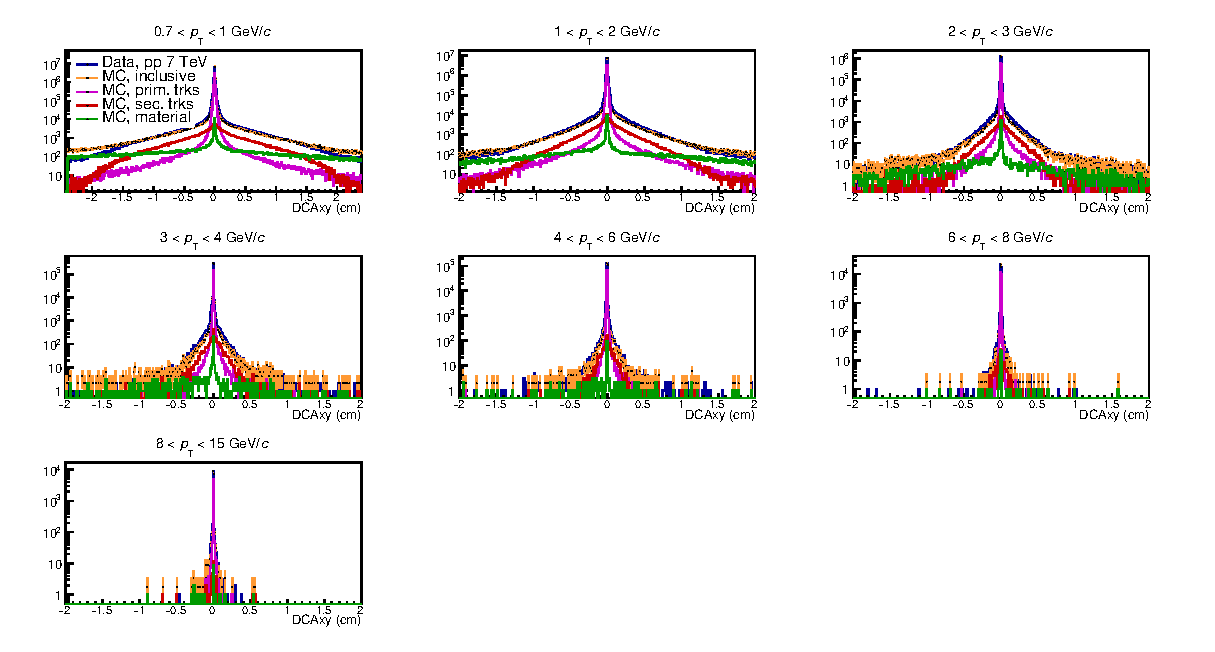
\includegraphics[width=.99\textwidth]{FigCap4/FitComponents.eps}
\caption{DCAxy distributions in data and in MC for primary and secondary tracks in different colours, in $\pt$ intervals from 0.5 to 15 $\Gevc$.}
\label{fig:DCAxyDataMCVsPt}
\end{center}
\end{figure}

\begin{figure}[!htb]
\begin{center}
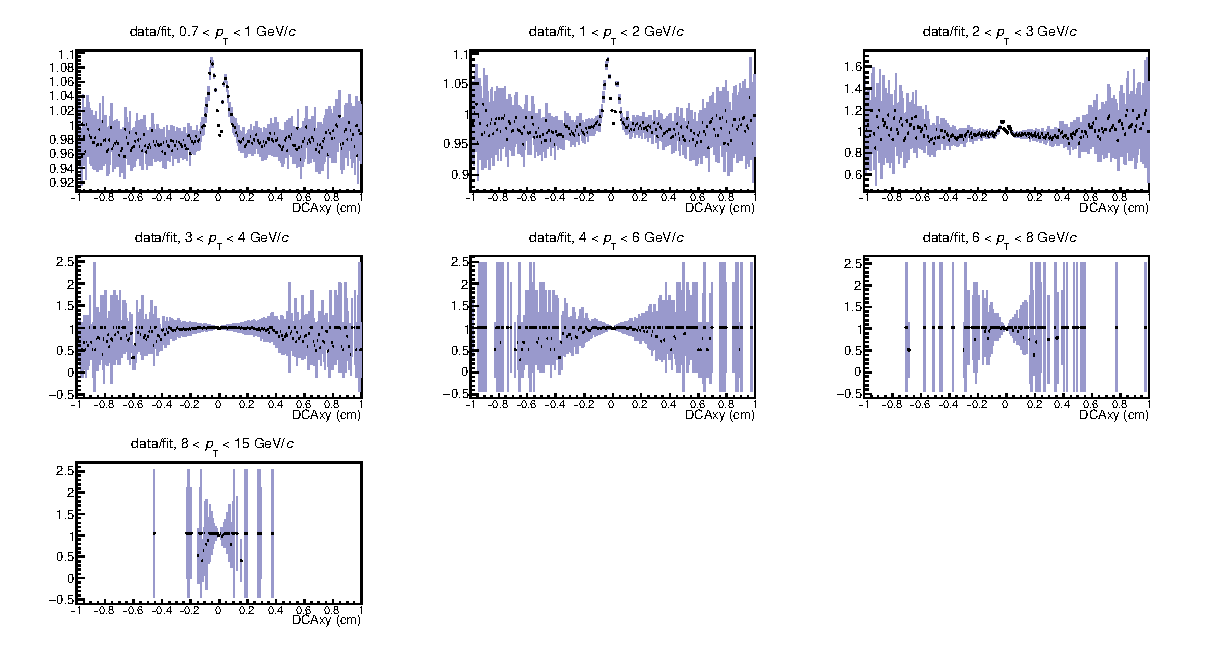
\includegraphics[width=.99\textwidth]{FigCap4/DataOverFit.eps}
\caption{Ratio of DCAxy distributions in data and in the fit result histograms, in $\pt$ intervals from 0.5 to 15 $\Gevc$.}
\label{fig:DCAxyRatioDataFitVsPt}
\end{center}
\end{figure}

\begin{figure}[!htb]
\begin{center}
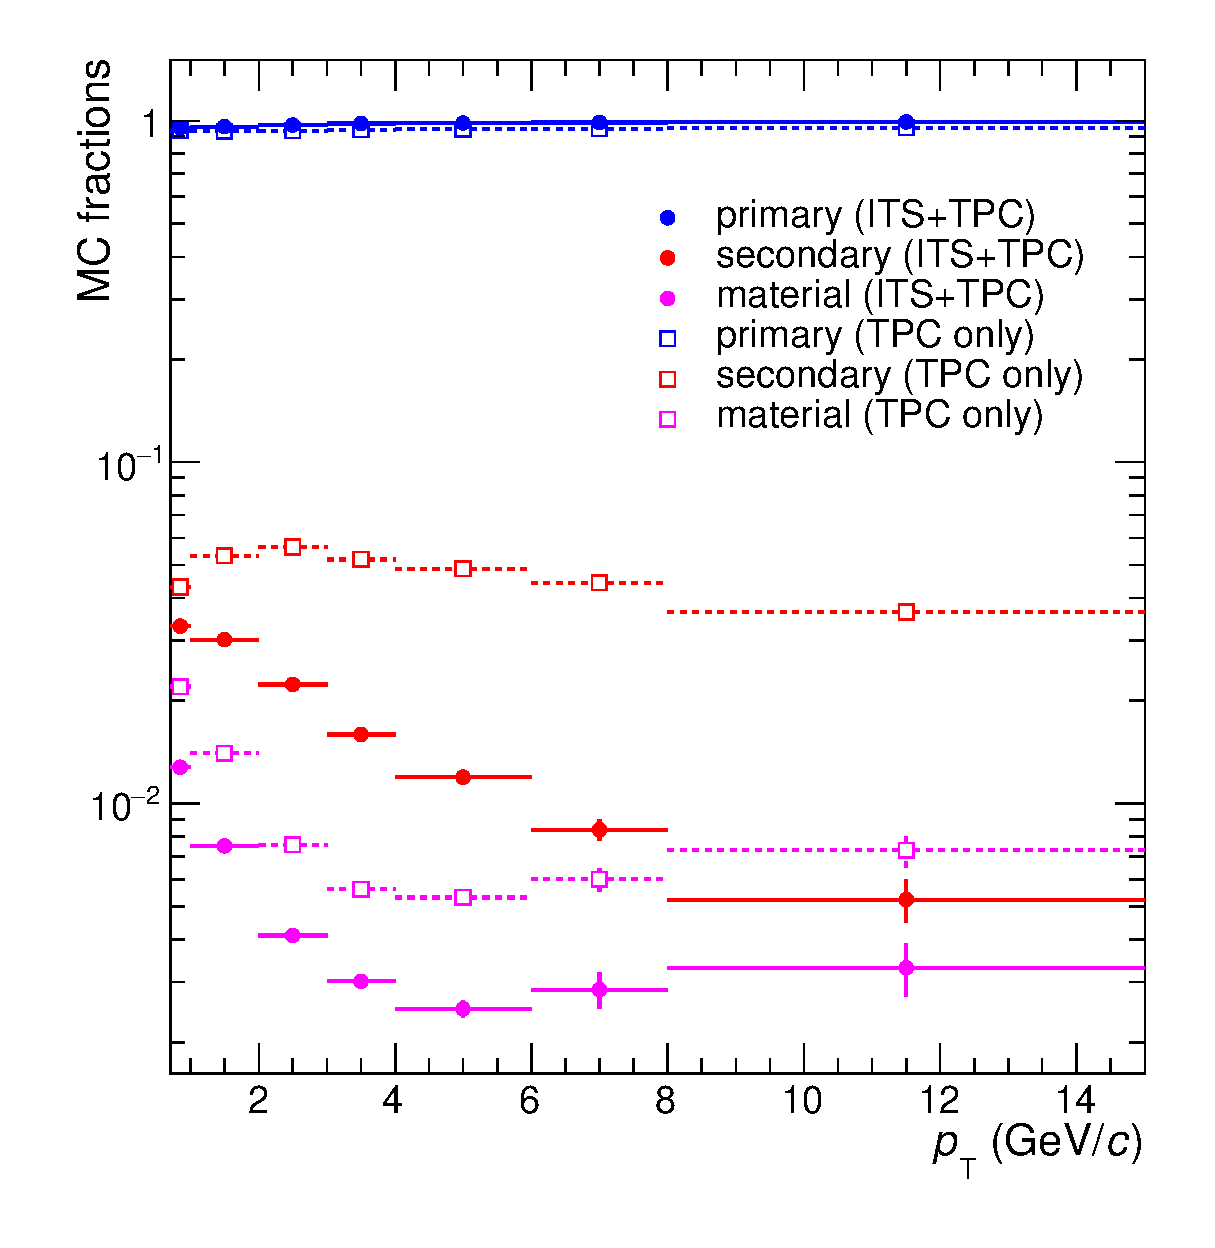
\includegraphics[width=.50\textwidth]{FigCap4/MCfractions_ESDTrOnly_VsPt_PiK.eps}
\caption{Example of fractions of primary and secondary tracks in MC requiring ITS-TPC or TPC only in different colours as a function of $\pt$.}
\label{fig:MCfractions}
\end{center}
\end{figure}

\begin{figure}[!htb]
\begin{center}
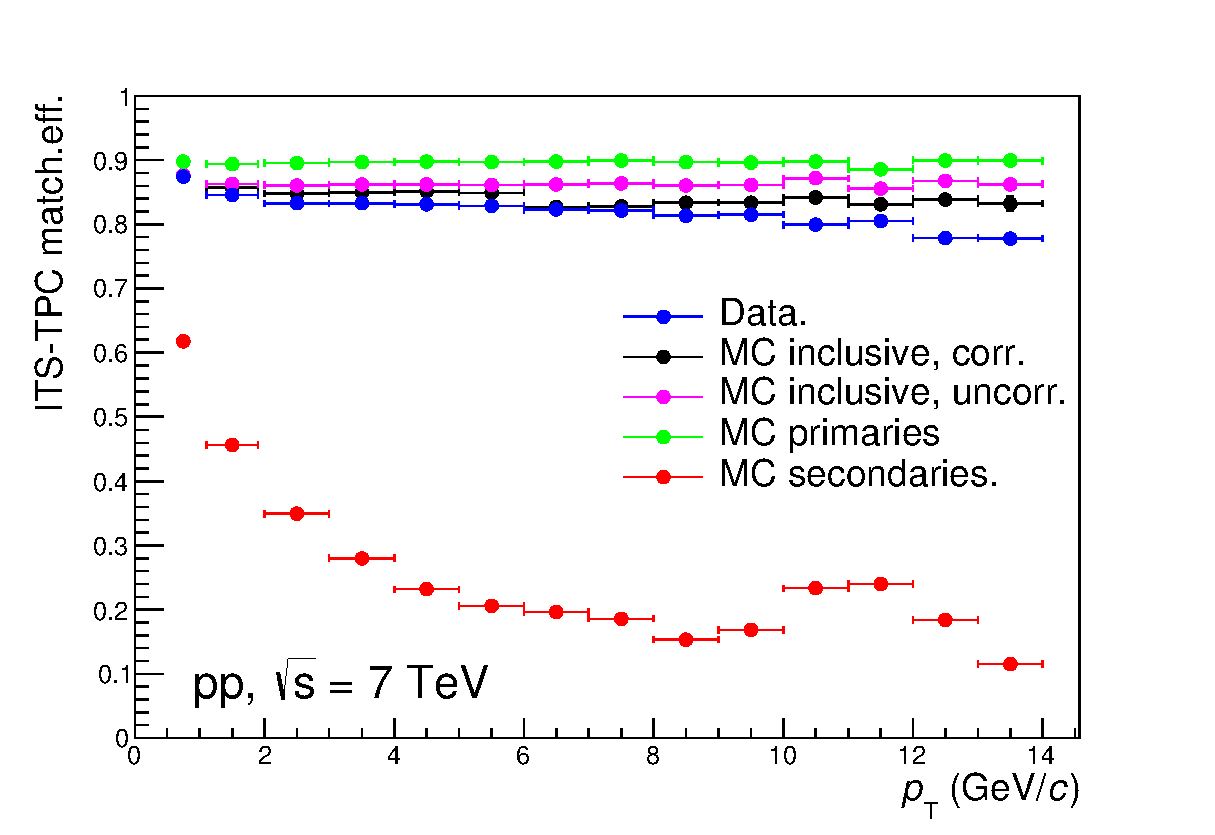
\includegraphics[height=7cm]{FigCap4/ITSTPCmatchEff_10bpass4_vsPt.eps}
\caption{Matching Efficiency as a function of $\pt$ for period b (left), and period d (right). The matching efficiency is shown for data (blu) for MC primaries and secondaries, separately (green and red), and for the MC corrected with the fraction of secondaries and primaries (black) Also the uncorrected MC is shown (magenta). }
\label{fig:CorrMatchEffVsPt}
\end{center}
\end{figure}

\begin{figure}[!htb]
\begin{center}
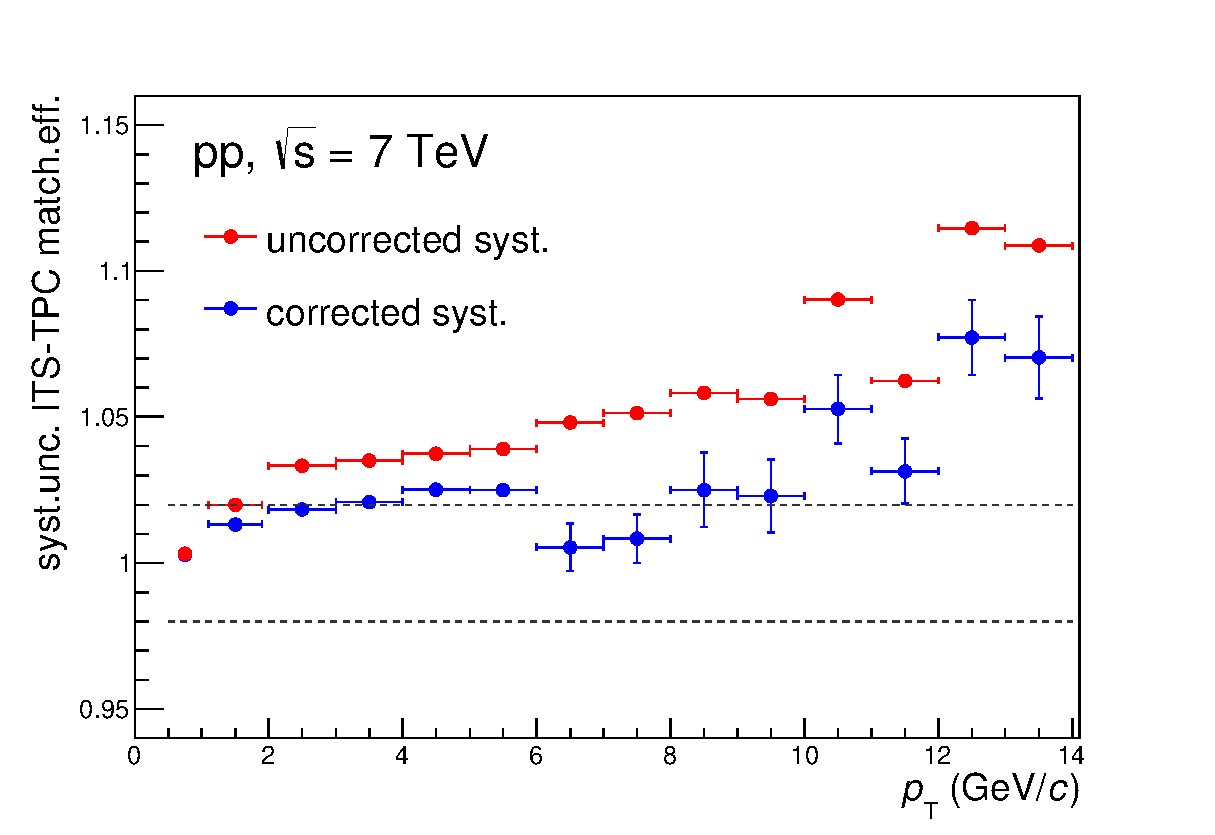
\includegraphics[height=7cm]{FigCap4/ITSTPCmatchEffSyst_10bpass4_vsPt.eps}
\caption{Matching Efficiency as a function of $\pt$ for period b (left), and period d (right). The matching efficiency is shown for data (blu) for MC primaries and secondaries, separately (green and red), and for the MC corrected with the fraction of secondaries and primaries (black) Also the uncorrected MC is shown (magenta). }
\label{fig:CorrMatchEffVsPt}
\end{center}
\end{figure}

\begin{figure}[!htb]
\begin{center}
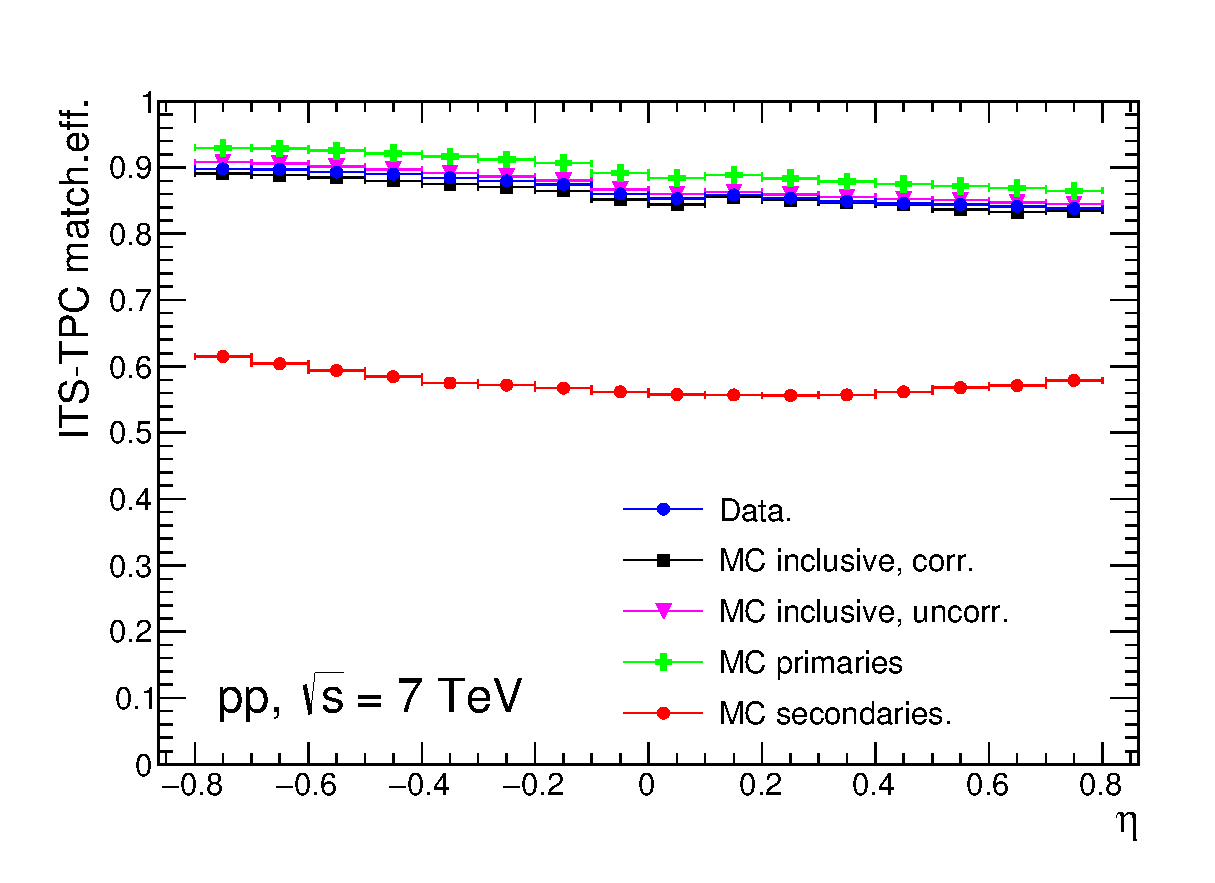
\includegraphics[width=.49\textwidth]{FigCap4/ITSTPCmatchEff_10bpass4_vsEta.eps}
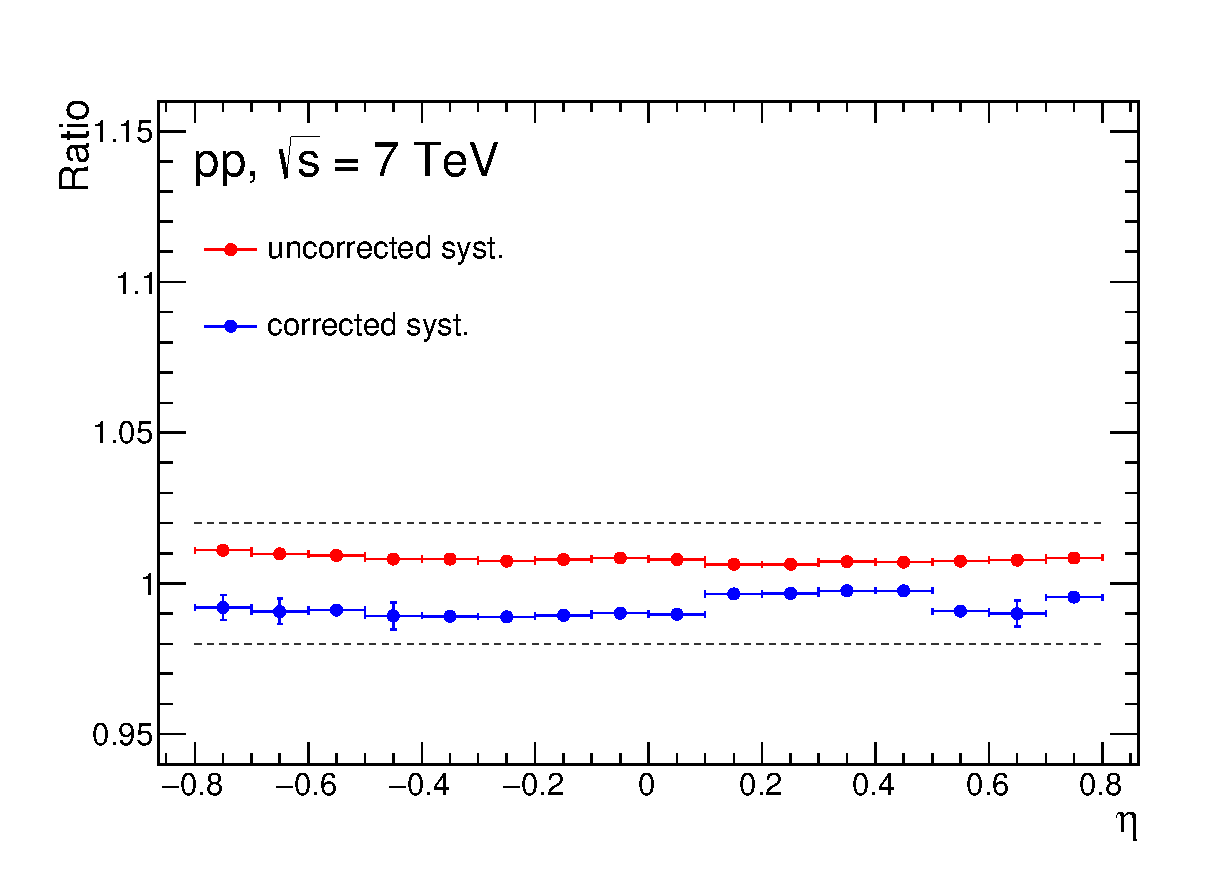
\includegraphics[width=.49\textwidth]{FigCap4/ITSTPCmatchEffSyst_10bpass4_vsEta.eps}
\caption{Matching Efficiency as a function of $\pt$ for period b (left), and period d (right). The matching efficiency is shown for data (blu) for MC primaries and secondaries, separately (green and red), and for the MC corrected with the fraction of secondaries and primaries (black) Also the uncorrected MC is shown (magenta). }
\label{fig:CorrMatchEffVsEta}
\end{center}
\end{figure}

\begin{figure}[!htb]
\begin{center}
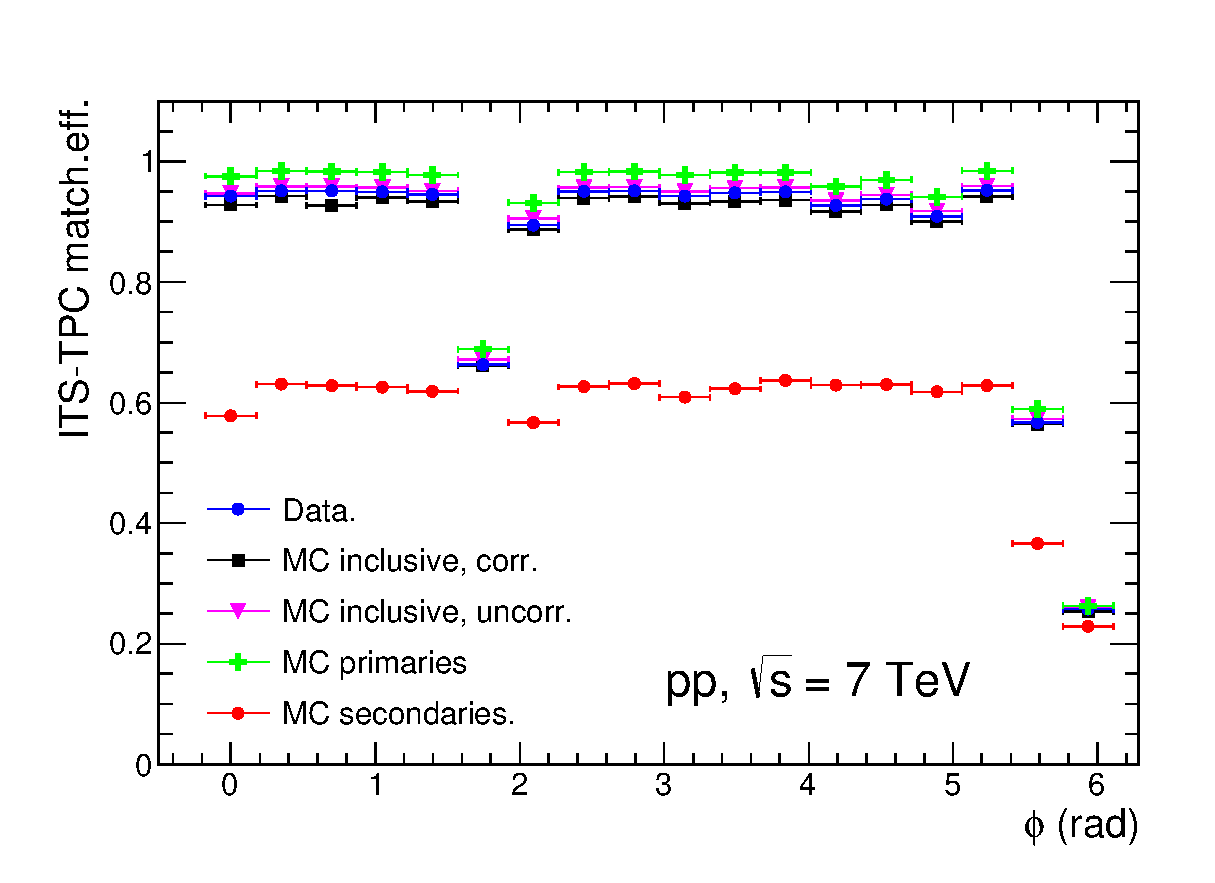
\includegraphics[width=.49\textwidth]{FigCap4/ITSTPCmatchEff_10bpass4_vsPhi.eps}
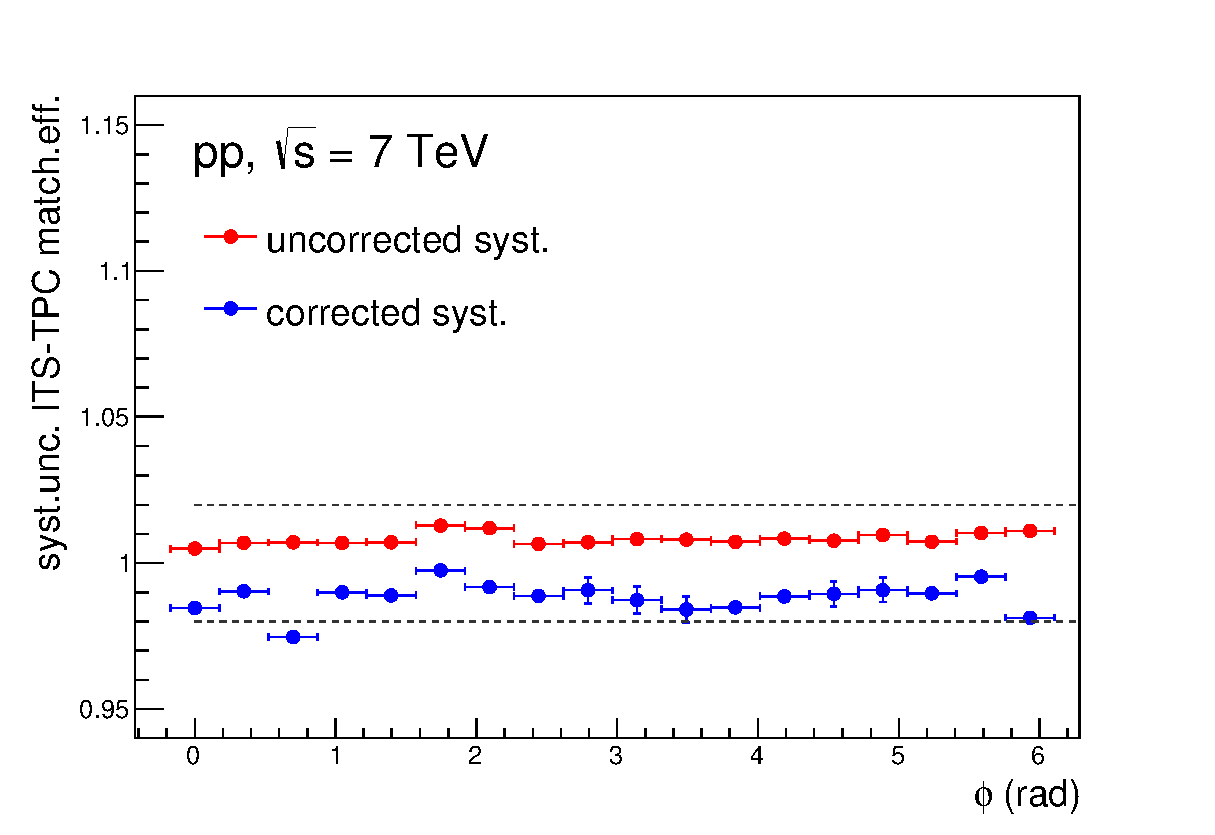
\includegraphics[width=.49\textwidth]{FigCap4/ITSTPCmatchEffSyst_10bpass4_vsPhi.eps}
\caption{Matching Efficiency as a function of $\pt$ for period b (left), and period d (right). The matching efficiency is shown for data (blu) for MC primaries and secondaries, separately (green and red), and for the MC corrected with the fraction of secondaries and primaries (black) Also the uncorrected MC is shown (magenta). }
\label{fig:CorrMatchEffVsPhi}
\end{center}
\end{figure}

\begin{figure}[!htb]
\begin{center}
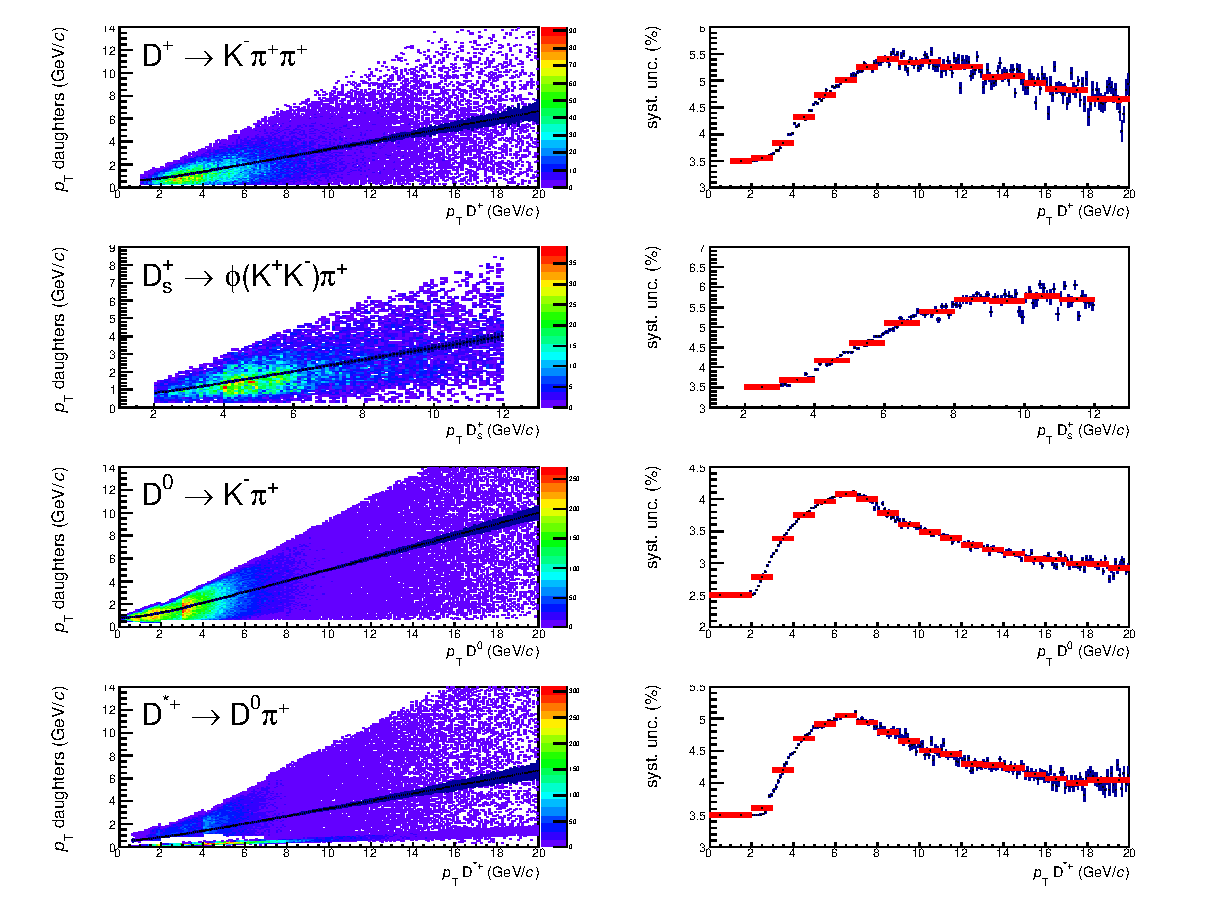
\includegraphics[width=1\textwidth]{FigCap4/FinalSystMEDmesons_ppPass4.eps}
\caption{Left column: scatter plot of daughter's $\pt$ versus D-meson $\pt$ for $\Dplus$, $\Ds$, $\Dzero$ and $\Dstar$ from top to bottom. Right column: final systematic uncertainties propagated at D-meson level after weighting for daughter's kinematics, as a function of $\pt$.}
\label{fig:SysMatchEffVsPhi}
\end{center}
\end{figure}

\subsection{B feed-down}
In the framework of D-meson analysis we currently use two different 
methods for the B feed-down subtraction, namely N$_{\rm b}$ and $f_{\rm c}$. 
The first method, used to give the central value for $f_{\rm prompt}$, 
needs as inputs for the calculations the FONLL predictions
for B-meson cross-sections and the Monte Carlo efficiency for B feed-down 
D mesons.
The second method, instead, takes as inputs FONLL predictions for both 
feed-down and prompt D mesons and their respective Monte Carlo efficiencies, 
as follows:\\
\begin{equation}
f^\prime_{\rm prompt} = \left( 	1 + 	\frac{({\rm Acc}\times\epsilon)_{{\rm feed-down}}}{({\rm Acc}\times\epsilon)_{{\rm prompt}}}	\cdot
		 \frac{ \left(\frac{{\rm d}^2 \sigma}{{\rm d}y \, {\rm d} \pt } \right)^{{\sf FONLL}}_{{\rm feed-down}} }{ \left(\frac{{\rm d}^2 \sigma}{{\rm d}y \, {\rm d} \pt } \right)^{{\sf FONLL}}_{ {\rm prompt} } } 
\right)^{-1} \, .
\label{eq:fc}
\end{equation}
\\We want to compare now FONLL predictions for heavy-flavored hadrons
 to the current available measurements of beauty and charmed 
 meson cross-sections at the LHC.
It is useful in order to decide whether to continue with the 
double-method strategy or to reduce to the N$_{b}$-only usage.
In Fig.~\ref{fig:Bmesons} the B$^{+}$, B$^{0}$, B$_{\rm s}$ and 
$\Lambda_{\rm b}$ cross-sections measured by CMS in pp collisions at 7 TeV
are compared with FONLL predictions.
The measurements lay within FONLL uncertainty bands in the case 
of non-strange B mesons. 
In Fig.~\ref{fig:LHCbBmesons}, measurements of B hadrons from 
LHCb in pp collisions at 7 TeV in the rapidity interval 
\mbox{2.0 $< y_{\rm cm} <$ 4.5}  are shown.
To scale FONLL predictions we used the fragmentation fraction values 
of b quarks into B hadrons measured by LHCb in the rapidity interval 
2.0 $< y_{\rm cm} <$ 4.5. Such measurements aim for an 
enhancement of bayon production at high rapidity with respect to 
mid-rapidity, in spite of a decrease of non-strange B-meson production. 
In Fig.~\ref{fig:LHCbBmesons}, starting from the top left figure, the 
comparison between LHCb B$^{+}$-meson cross-section and FONLL
 curve shows good agreement.
The top right plot shows instead a better agreement for 
B$_{\rm s}$-meson data from LHCb with FONLL, in a wider 
$p_{T}$ range than those of CMS.
The CMS and LHCb B$_{\rm s}$-meson cross-sections in 
8 $< p_{\rm T} <$ 50 GeV/$c$ as a function of y are shown in 
the bottom left plot, together with the FONLL predictions in the 
two different rapidity intervals. For the CMS data, two cases are 
reported, one obtained using the current (2015) PDG value for 
BR(B$_{\rm s} \rightarrow J/{\rm \psi} ~\Phi$),
the other obtained using the 2010 PDG value, referenced in the 
CMS paper. As regards $\Lambda_{\rm b}$ cross-section 
(bottom right plot), FONLL provides a shape which is compatible
 with LHCb data, provided a rescaling of a factor 2, which may account
  for uncertainties on the determination of the BR($\Lambda_{b} \rightarrow J/\psi {\rm p K}$) 
  used by LHCb to provide the cross-section.
In Fig.~\ref{fig:Dmesons} we can see the $J/\psi$ from beauty-decay 
cross-section in pp collisions at 7 TeV measured by LHCb, and the 
D$^{+}$-, D$^{0}$-, D$^{*+}$-meson cross-sections at 7 TeV by ALICE.
In the case of $J/\psi$ meson, FONLL provides a good description of 
the 7 TeV data, as well as for the 8 TeV ones (not shown here). 
The D-meson results show that 
experimental data sistematically lay on the upper edge of FONLL uncertainty 
band, thus charm production being underestimated by FONLL.\\
Considering that:
\begin{itemize}
\item FONLL provides a good description of B$^{+}$-, B$^{0}$-meson 
cross-sections at 7 TeV both at mid- and forward rapidity and of 
$J/{\rm \psi}$-meson cross-section at forward rapidity;
\item FONLL provides a good description also for the 
B$_{\rm s}$-meson and $\Lambda_{\rm b}$-baryon cross-sections 
at forward rapidity where data are available in a wider $p_{T}$ range 
than at mid-rapidity, allowing for a safer comparison. The rescaling 
of the shape for the $\Lambda_{\rm b}$ cross-section could be due 
to the uncertainty on the branching ratio
of the channel used by LHCb in the analysis,
\end{itemize}
the calculation of $f_{\rm prompt}$ with the $N_{\rm b}$ method is then fully justified.
The $f_{\rm c}$ method, instead, would suffer from the 
underestimation of charm production at the
LHC energies. It is reasonable to conclude, thanks to the available 
measurements, that $f_{\rm c}$ would artificially introduce a bias if 
used to subtract the beauty feed-down component.
Besides, this choice will give benefit to our feed-down systematic 
estimate. In Tab.~\ref{tab:systFD} we can see an example for the D$_{\rm s}$.

\begin{table}[tbh!]
\centering
\begin{tabular}{|clc|c|c|c|} 
\hline
& \multicolumn{2}{c|}{N$_{\rm b}$ + $f_{\rm c}$} & \multicolumn{2}{c|}{N$_{\rm b}$ only}\\
\hline
$p_{\rm T}$ (GeV/c) & +systFD & -systFD & +systFD & -systFD \\
\hline
2-4        & 4.1\% & 17.0\% & 4.1\% & 4.6\%\\
4-6        & 3.7\% & 10.2\% & 3.7\% & 4.7\%\\
6-8        & 3.8\% & 10.0\% & 3.8\% & 4.8\%\\
8-12        & 4.0\% & 9.0\% & 4.0\% & 4.8\%\\
\hline
\end{tabular}
\caption{Comparison of the systematic uncertainty on the feed-down subtraction for the D$_{\rm s}$ meson.} 
\label{tab:systFD}
\end{table}

\subsection{Generated $\pt$ shape}

The systematic effect on the efficiency extracted from the simulations due to
the generated $\pt$ shape of D mesons was tested by computing the efficiency
with and without using in the AliCFTaskVertexingHF task the $\pt$-dependent 
weights  that allow us to correct for the difference between the $\pt$ 
spectrum of generated $\Dzero$ mesons in the LHC10f7a production and the 
prediction from FONLL.


\begin{table}[!tb]
\centering
\begin{tabular}{l|ccccc|}
 \hline 
  & \multicolumn{4}{c|}{$\pt$ interval ($\GeV/c$)}\\
 & 2--4 & 4--6 & 6--8 & 8--12\\
\hline
Raw yield extraction & 5\%& 5\%& 5\%& 5\%\\
Topol. sel. efficiency & 7\%& 7\%& 7\%& 7\%\\
Tracking efficiency & 5\%& 5.5\% & 6\% & 6\%\\
PID efficiency & 7\%& 7\%& 7\%& 7\%\\
MC $\pt$ shape   &3\%&3\%&2\%&2\%\\
Feed-down from B & $^{+4.1\%}_{-4.6\%}$& $^{+3.7\%}_{-4.7\%}$& $^{+3.8\%}_{-4.8\%}$& $^{+4.0\%}_{-4.8\%}$\\
Luminosity  
  & \multicolumn{4}{c|}{3.5\%} \\
\hline 
\end{tabular}
\caption{Relative systematic uncertainties on the $\pt$-differential production
cross section of prompt $\Ds$ mesons.}
\label{tab:SystDs}
\end{table}

\section{Results}
The $\pt$-differential cross sections for prompt D-meson production
are reported in this section.
In Fig., the $\Dzero$-meson cross section
from this analysis is compared to the published one based on the analysis of 
the pass2 reconstruction of the 2010 pp sample and to FONLL calculations.
The ratios to FONLL predictions for the new and the published analyses
and of the new result to the published one are also reported.
The comparison of the relative statistical and systematic uncertainties
on the new and on the published (pass2) results are shown in 
Fig..
The statistical uncertainties on the new results are slightly reduced as
compared to the published one, while there is a substantial reduction, 
by a factor 1.5--3 depending on $\pt$, of the systematic uncertainties.



The $\Ds$-meson $\pt$-differential cross sections are shown in 
Fig.~\ref{fig:CrossSecDs2vs4}, where they are compared to the
published results based on the pass2 reconstruction.
The comparison to the predictions from pQCD calculations with the
GM-VFNS approach and the LO $k_{\rm T}$ factorization 
algorithm are shown in Fig.~\ref{fig:CrossSecDsvsGMVFNS}.


\begin{figure}[!htb]
\begin{center}
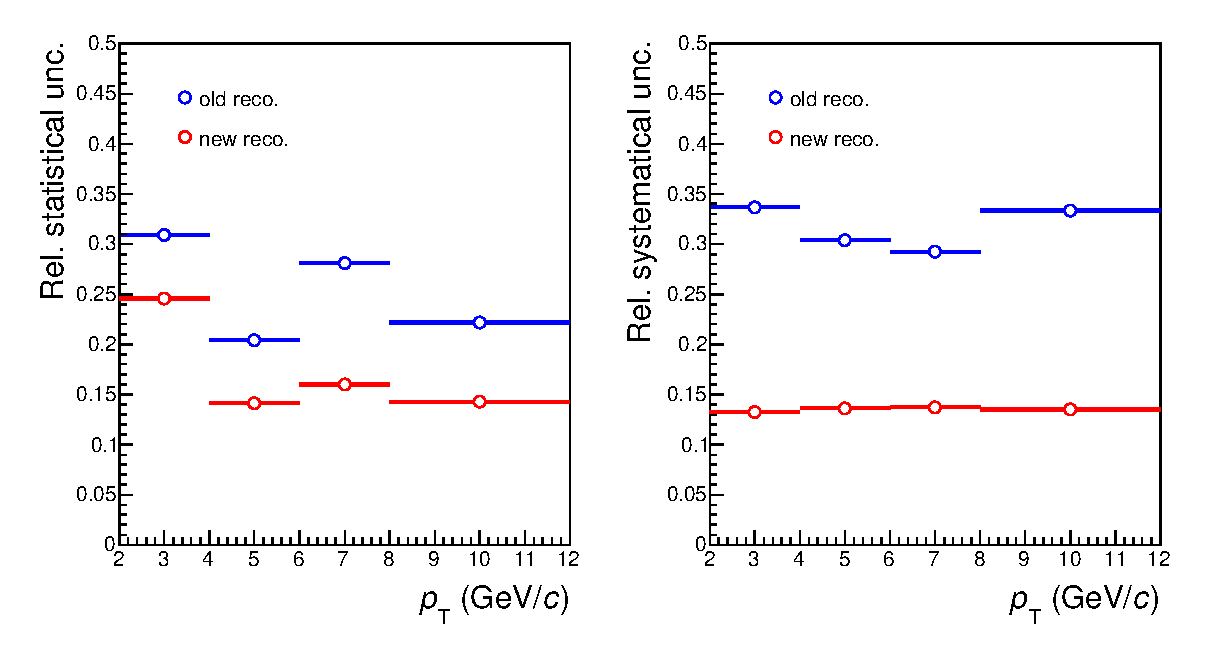
\includegraphics[width=.99\textwidth]{FigCap4/uncertainties_pass2_pass4.eps}
\caption{Comparison of statistical and systematic uncertainty on $\Ds$-meson
cross section in the pass2-based publication and this re-analysis.}
\label{fig:CrossSecDs2vs4}
\end{center}
\end{figure}

\begin{figure}[!htb]
\begin{center}
%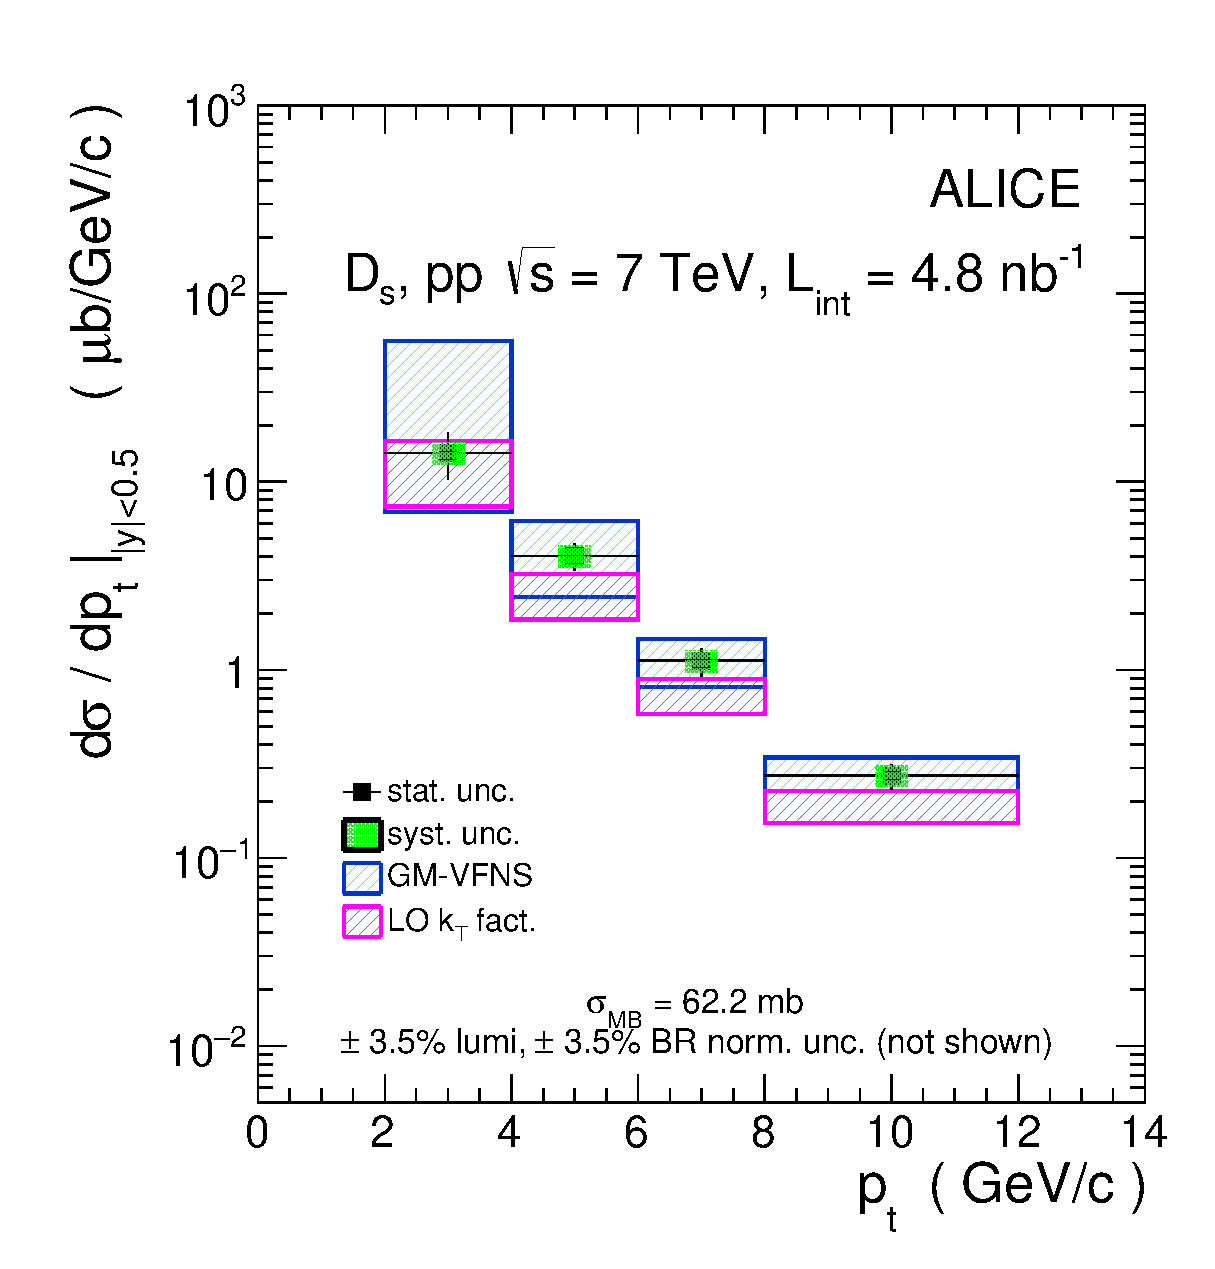
\includegraphics[width=.48\textwidth]{FigCap4/DsCrossModel.eps}
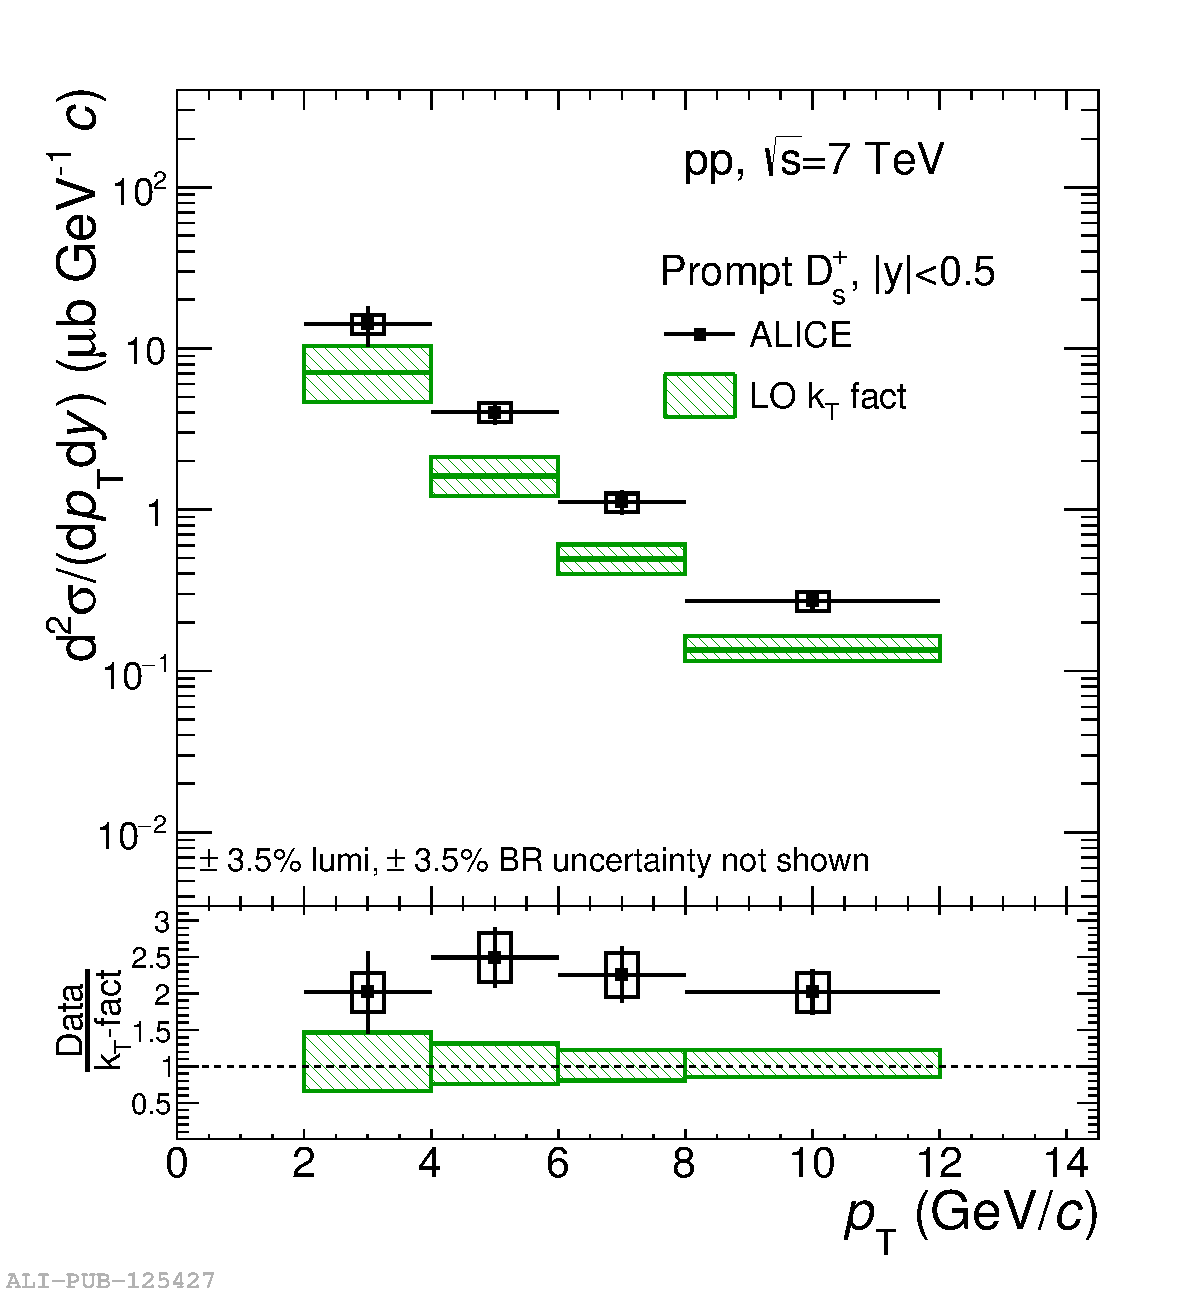
\includegraphics[width=.48\textwidth]{FigCap4/DsppCrossSecVsKtFactAndRatio.pdf}
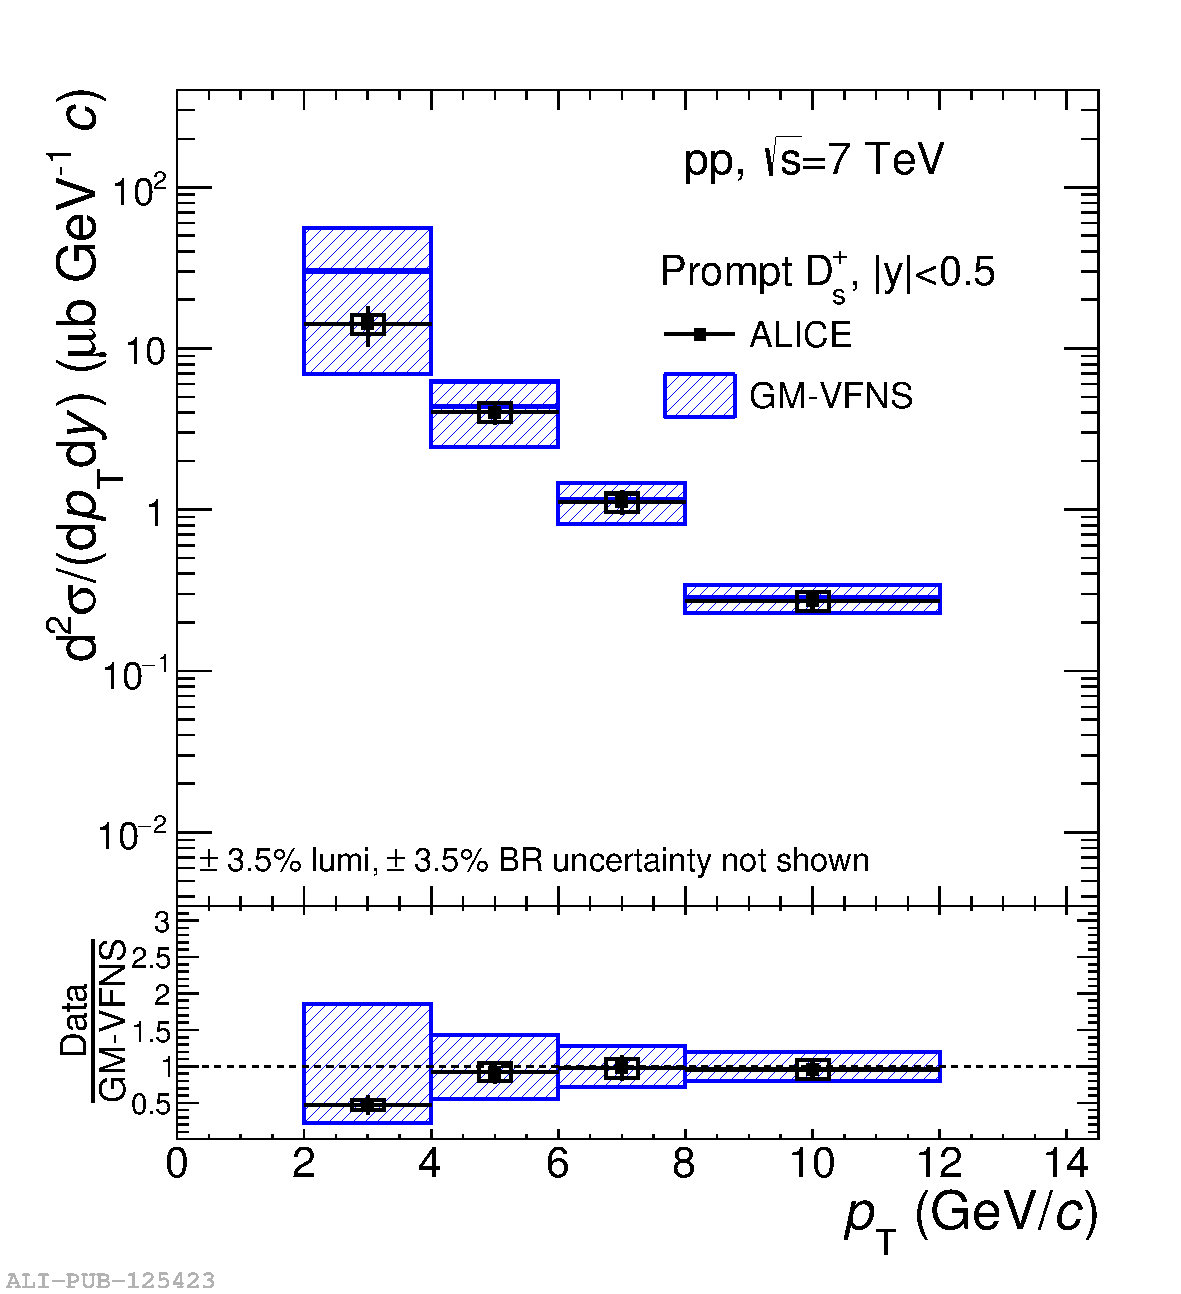
\includegraphics[width=.48\textwidth]{FigCap4/DsppCrossSecVsGMVFNSAndRatio.pdf}
\caption{Prompt $\Ds$-meson production cross section compared
to GM-VFNS calculations.}
\label{fig:CrossSecDsvsGMVFNS}
\end{center}
\end{figure}


In Fig.~\ref{fig:RatiosPass4}, the
 $\Dplus$/$\Dzero$, $\Ds$/$\Dzero$, $\Ds$/$\Dplus$ 
 meson production in pp pass4 are shown
as a function of $\pt$.
In Fig.~\ref{fig:RatiosPass2Pass4}, the same ratios are 
shown compared to published measurements in pass2, with an effective reduction of 
statistical and systematic uncertainties. 

\begin{figure}[!htb]
\begin{center}
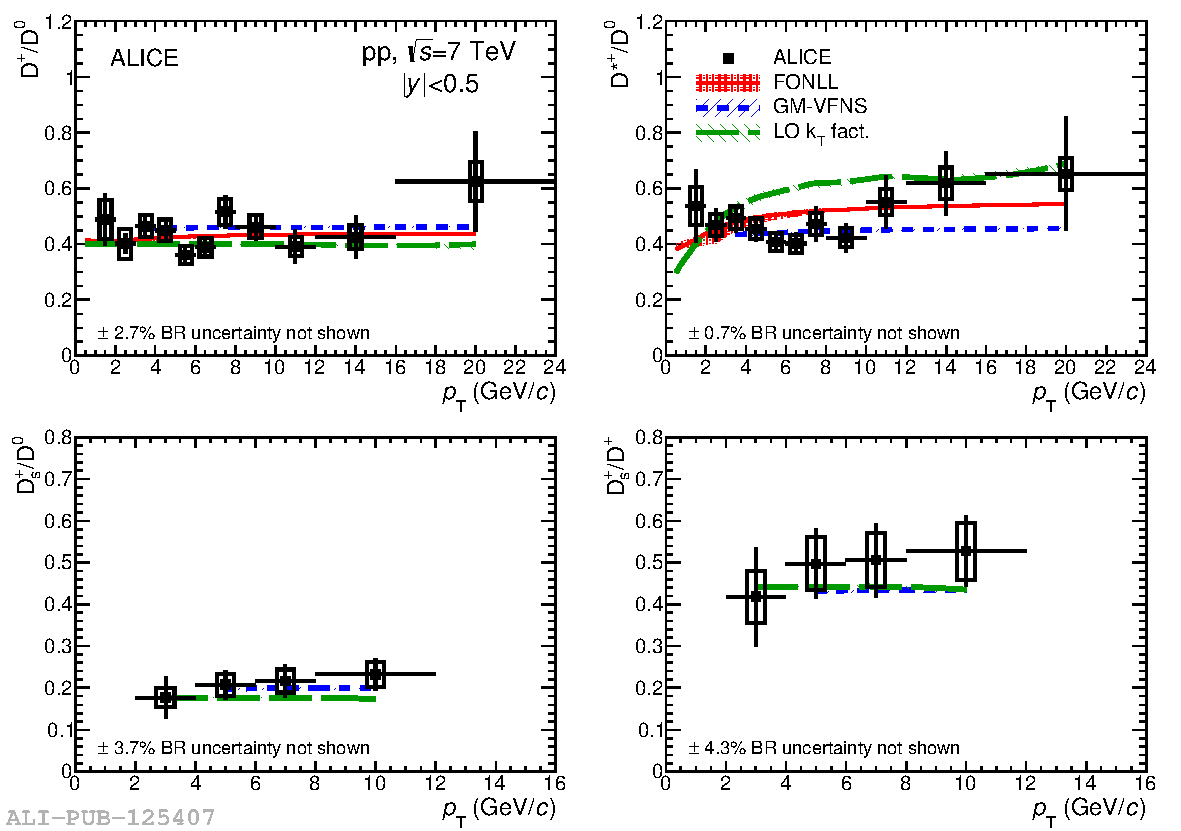
\includegraphics[width=1\textwidth]{FigCap4/DmesonRatiosVsModels.pdf}
\caption{D-meson production ratios in pp pass4 compared to the published results in pass2.}
\label{fig:RatiosPass2Pass4}
\end{center}
\end{figure}


